\documentclass{article} % For LaTeX2e
\usepackage{nips13submit_e,times}
\usepackage{geometry}
\usepackage[toc,page]{appendix}
\usepackage{listings}
\usepackage[hyphens]{url}
\usepackage{bbm}
\usepackage{amsfonts, amssymb}
\usepackage{alltt}
\usepackage{multirow, caption}
\usepackage{algorithm}
\usepackage{amsmath}
\usepackage{graphicx}
\usepackage[noend]{algpseudocode}
\usepackage{etoolbox}
\usepackage{hyperref}
\usepackage{fancyvrb}
\usepackage{tgcursor}
\usepackage{longtable}
\usepackage{authblk}
\usepackage{amsthm}
\usepackage{wrapfig}
\usepackage{bm}
\usepackage{breqn}
\usepackage{textcomp, listings,multicol}

\newcommand\userinput[1]{\textbf{#1}}
\newcommand\comment[1]{\textit{#1}}
\newcommand\stdout[1]{\textsl{#1}}

\makeatletter
\preto{\@verbatim}{\topsep=0pt \partopsep=0pt }
\makeatother

% Tweak algorithmic package.
\renewcommand{\algorithmicrequire}{\textbf{Input:}}
\renewcommand{\algorithmicensure}{\textbf{Output:}}

% Tweak itemize
\def\labelitemi{--}

% Definition, Lemma, Theorem...
\theoremstyle{definition}
\newtheorem{defn}{Definition}

\theoremstyle{theorem}
\newtheorem{lemma}{Lemma}
\newtheorem{thm}{Theorem}

\theoremstyle{remark}
\newtheorem*{remark}{Remark}

\theoremstyle{remark}
\newtheorem{remk}{Remark}
\lstset{ %
  backgroundcolor=\color{white},   % choose the background color
  basicstyle=\footnotesize,        % size of fonts used for the code
  breaklines=true,                 % automatic line breaking only at whitespace
  captionpos=b,                    % sets the caption-position to bottom
  commentstyle=\color{mygreen},    % comment style
  escapeinside={\%*}{*)},          % if you want to add LaTeX within your code
  keywordstyle=\color{blue},       % keyword style
  stringstyle=\color{mymauve},     % string literal style
}

%%%%%%%%%%%%%%%%%%%%%%%%%%%%%%%
%% Definition for code appendix

% Copy code not line number
\usepackage{accsupp}
\newcommand*{\noaccsupp}[1]{\BeginAccSupp{ActualText={}}#1\EndAccSupp{}}
% end

\lstdefinestyle{shared}
{
    numbers=left,
    numbersep=1em,
    numberstyle=\tiny\color{red}\noaccsupp,
    frame=single,
    framesep=\fboxsep,
    framerule=\fboxrule,
    rulecolor=\color{red},
    xleftmargin=\dimexpr\fboxsep+\fboxrule\relax,
    xrightmargin=\dimexpr\fboxsep+\fboxrule\relax,
    breaklines=true,
    tabsize=2,
    columns=flexible,
}


\lstdefinestyle{python}
{
    style=shared,
    language={Python},
    %alsolanguage={[Sharp]C},
    basicstyle=\small\tt,
    keywordstyle=\color{blue},
    commentstyle=\color[rgb]{0.13,0.54,0.13},
    backgroundcolor=\color{cyan!10},
    morekeywords={
        Console,
        WriteLine,
        int,
    },
}

\lstnewenvironment{python}
{\lstset{style=python}}
{}


\definecolor{mygreen}{rgb}{0,0.6,0}
\definecolor{mygray}{rgb}{0.5,0.5,0.5}
\definecolor{mymauve}{rgb}{0.58,0,0.82}

%%%%%%%%%%%%%%%%%%%%%%%%%%%%%%%%%%%%%%%%%%%
%%% Main Body of Report
%%%%%%%%%%%%%%%%%%%%%%%%%%%%%%%%%%%%%%%%%%%


%%%%%% Title Page
\title{Password Guessability with Markov Model\\Final Report}
\author[1]{Derek Tzeng}
\author[1]{Yiming Zong}
\affil[1]{School of Computer Science, Carnegie Mellon University}

\renewcommand\Authands{ and }
\nipsfinalcopy % Uncomment for camera-ready version

% Line spacing for comfortable reading
\linespread{1.125}
\begin{document}

% Title
\maketitle

% Paper Abstract
\begin{abstract}
    \par\quad As text-based passwords remain the prevalent method of authentication, it is important to understand the security level of a password in order to help users create strong passwords. Markov model is a preferred method for professionals to crack passwords, and it is therefore helpful to learn how many trials it takes to guess a password with such model. In the report, we first survey existing research on password security and present our design of Markov look-up table that reduces the guessing time significantly compared to naive enumeration. Afterwards, we analyze the performance of our algorithm and discuss some key takeaways including time-space tradeoff and usability. Eventually, we point out potential directions for future research, including alternative models and potential applications.
\end{abstract}

\textbf{Keywords:} Authentication, Password strength, Cryptanalysis, Markov model
\vspace{\fill}
\pagebreak

%%%%%%%%%%%%%%%%%%%%%%%%%%%%%%%%%%%%%%%%%%%%%%%%%%%%%%%%
%%%%% Main Body Starts
%%%%%%%%%%%%%%%%%%%%%%%%%%%%%%%%%%%%%%%%%%%%%%%%%%%%%%%%
\section{Introduction}

\subsection{Background \& Motivation}
\par\quad Text-based passwords are the most commonly used method for authentication, and will very likely remain so for the foreseeable future \cite{persistence}. While passwords offer an intuitive, low-cost, and convenient way for users to protect personal information, they are vulnerable to various attacks. A typical model is when the attacker obtains a database of hashed passwords and is able to crack the passwords however they wish. The clear-text passwords are then used to compromise personal information, which has caused significant financial and social impacts in the past \cite{money}.

\par\quad Nowadays, hashes are often applied to passwords for server-side storage, such that even when an attacker obtains the password database, it is memory- and/or computationally-intensive to crack even a single hash -- usually the attacker needs to enumerate \textit{all} potential passwords per some heuristic and check if the guess is correct \cite{bcrypt}. However, server-side security measures do not stop users from selecting ``common'' passwords \cite{easypass}, which allows the attacker to guess correctly in a manageable number of trials. Therefore, it is important for system administrators to instruct users to create secure passwords.

\par\quad In order to define a ``secure password'', it is natural to measure password strength in terms of the number of trials an attacker makes before getting to a particular password. Previous studies have shown that password strength can be estimated with automated guessing when the model is tuned carefully (\cite{guessability}, \cite{probabilistic}). And, this is the approach that our study takes.

\par\quad Among the password enumeration heuristics, Markov model has proved effective in traversing more likely passwords earlier in the guessing process (\cite{omen}, \cite{guessability}), and hence is popular among attackers. In this study, we aim to measure the strength of a password by calculating the number of attempts an attacker makes before getting to it with Markov model. We hope that our study can give system administrators more insights on the security measure of passwords and provide a new potential metric for password meters.

\subsection{Report Organization}
\par\quad In \emph{Section 2}, we first present a comprehensive literature review on previous work in password security that is relevant to our study. The aim is to introduce readers to the area of password security without assuming much prior knowledge. In \emph{Section 3}, we will propose our algorithm and implementation for the Markov look-up table, along with discussions on parameter tuning and input selection. In \emph{Section 4}, we will analyze the performance and accuracy of our approach, followed by key takeaways of our study in \emph{Sections 5}. Eventually, we will discuss potential future work in \emph{Section 6}.

%%%%%%%%%%%%%%%%%%%%%%%%%%%%%%%%%%%%%%%%%%%%%%%%%%%%%%%%%%%%%%%%%%%%
%%%%%%%%%%%%%%%%%%%%%%%%%%%%%%%%%%%%%%%%%%%%%%%%%%%%%%%%%%%%%%%%%%%%
\section{Previous Work}
\par\quad The topic of password security has appeared in academic research since passwords were first used for authentication purposes in modern systems. Existing research in this area can be roughly divided into the following categories:
\begin{itemize}
    \renewcommand\labelitemi{--}
    \item Users' choice of passwords (\cite{easypass}, \cite{measureup}, \cite{addbang}): This category focuses on how to encourage or enforce users to choose ``strong'' passwords. Existing studies cover many different fields, ranging from algorithmic design \cite{easypass} to user studies \cite{measureup}.

    \item Security measures for storing passwords (\cite{PKCS}, \cite{bcrypt}, \cite{scrypt}): This category involves designing secure methods for service providers to store and validate passwords, such that even when the hashed passwords are leaked from the server, it is computationally hard to recover clear-text passwords. Most commonly used algorithms include bcrypt \cite{bcrypt} and PBKDF2 \cite{PKCS}.
    
    \item Enumeration model for cracking passwords (\cite{omen}, \cite{john}, \cite{probabilistic}, \cite{timespace}, \cite{passmodel}, \cite{PCFG}): Studies in this category are in the perspective of attackers -- they design and compare different password probability models including Markov model (\cite{omen}, \cite{probabilistic}, \cite{timespace}), probabilistic context-free grammar (PCFG) \cite{PCFG}, and word mangling rules \cite{john}. The purpose is to crack common passwords from hashes efficiently.
    
    \item Measuring the security of passwords (\cite{adaptive markov}, \cite{empirical}, \cite{probframework}, \cite{againagain}, \cite{guessability}): This category extends from the results in the previous category and concludes what types of passwords are the ``most secure'' under various attacks. Factors considered include password policy \cite{againagain}, Shannon entropy \cite{adaptive markov}, and similarity to natural language \cite{empirical}.
\end{itemize}

\begin{wrapfigure}{r}{0.5\textwidth}
    \vspace{-20pt}
    \begin{center}
        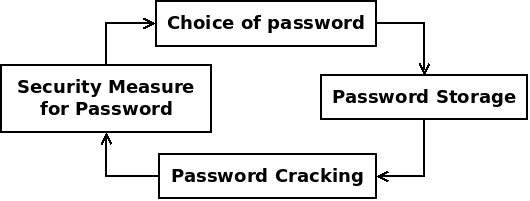
\includegraphics[width=0.48\textwidth]{diag/categories.png}
    \end{center}
    \vspace{-5pt}
    \caption{Categories of Password Security Research}
    \vspace{-0pt}
    \label{fig:categories}
\end{wrapfigure}

\par\quad Note that the four categories above form a causal chain (Figure \ref{fig:categories}) that drives password security forward: Users choose passwords for authentication purposes, and service-providers store the passwords securely. Intruders then attempt to crack the stored passwords, prompting the need for analyzing the security level of passwords. Eventually, the results of password analyses give rise to password policies and password strength meters, which in turn help users create more secure passwords.

\par\quad For the remainder of the section, we will present a literature review for each of the four categories above. Special focus will be given to the last two categories due to their relevance to our main contribution.

%%%%%%%%%% Use [1] [1] [1]

\subsection{Choice of Passwords}
\par\quad Passwords have been commonly used for authentication purposes for at least 35 years (\cite{history}, \cite{persistence}), and choosing passwords has always involved a trade-off between \emph{security} and \emph{convenience} -- a ``weak'' password is easy for users to remember and type, yet also easier for adversaries to crack. In response to this, research in this category mainly focuses on measures to encourage users to pick strong passwords and discourage users from picking weaker ones.

\par\quad Various studies focus on commonly used \emph{proactive password checker}, where a system can choose to accept or reject a password based on its approximated strength. The most common heuristics used today include NIST, Google, and Microsoft password checker, each of which considers a combination of length, character composition, and dictionary test \cite{adaptive markov}. Despite the popularity of proactive checkers, their effect is debated, as \cite{empirical} notes that users usually pick passwords \emph{just} secure enough to pass the checker, and stringent password checkers are likely to annoy users \cite{addbang}. Nonetheless, \cite{measureup} concludes a positive relation between the strength of password checker and the security of passwords chosen.

\par\quad Meanwhile, some other studies focus on algorithms for such password checkers. \cite{easypass} proposes a space-efficient and secure implementation of dictionary filter using a bloom filter, and \cite{adaptive markov} builds an adaptive password strength meter with Markov model in order to measure the security of a password based on existing ones.

\subsection{Security of Password Storage}
\par\quad Once a password is chosen by the user, it needs to be stored in some form for authentication purposes. Meanwhile, user credential databases can be vulnerable to attacks, a most famous example of which is \emph{SQL injection attack} \cite{SQL injection}. Hence, there has been ongoing studies on storing the obscured passwords on the database as \emph{cryptographic hashes} (\cite{PKCS}, \cite{bcrypt}, \cite{scrypt}), such that attackers cannot get the clear-text passwords directly. For sake of brevity, we will only discuss the common characteristics of the hashes instead of their implementation details, as follows:

\begin{enumerate}
    \item It should be extremely difficult to calculate a plain-text message whose hash matches a given hash. As a recent example, to crack a 10-char, scrypt-hashed\footnote{The cost factor used in the analysis is $11$, which is common in real-world settings at the time of writing.} password within a year would incur an estimated hardware cost of \$48 billion, whereas the typical hashing time is within $100$ms in consumer-grade CPUs \footnote{The CPU used by the study is one core of 2.5 GHz Intel Core 2 Duo processor.}\cite{scrypt}. This property helps protect the actual passwords even when the authentication database is compromised.

    \item It should be easy to calculate the hash of a clear-text message. This property is important since whenever a user creates a new account or authenticates to a service, hashed passwords need to be computed. This allows password-based authentication schemes to be scalable and affordable \cite{persistence}.
\end{enumerate}

\par\quad Meanwhile, as the computing power of machines has evolved exponentially over time \cite{moore}, the hashing schemes are constantly being challenged as the speed of cracking algorithms increases. In response to that, many prevalent hashing schemes incorporate tunable parameters that can maintain the ``relative strength'' of the scheme over time. For example, both scrypt and bcrypt have a notion of \emph{cost factor}, which determines the number of hashing rounds. As time goes on, the recommended cost factor increases to match up with the speedup of hardwares. On the contrary, some hashing schemes (e.g. MD5 crypt) do not have such notion, and over time its security has been greatly compromised\footnote{According to \cite{john-benchmark}, John the Ripper can crack MD5 crypt at 1953K hashes per second on a 128-core server.}.

\par\quad As an ending note on terminology, notice that in the discussion above we avoided using the term ``encryption''. The reason is that encryption schemes almost always have corresponding decryption routines, which give the authentication system another vulnerability for exploits. On the other hand, the approaches we discussed above are all cryptographic hashes instead.

\subsection{Common Password Enumeration Heuristics}
\par\quad In the previous section, we noted that it is technically impossible to directly invert a password hash back to the clear-text password. Hence, in real-world attacks, adversaries will usually enumerate a list of potential passwords and check if their hashes match the desired one. Since the search space is inevitably large, the order of guessing can greatly affect the performance of the enumeration routine \cite{empirical}. In this section, we will survey the most common password enumeration techniques used by password security professionals.

\subsubsection{Brute-Force}
\par\quad Brute-Force is the most naive enumeration scheme of the four we discuss, and it is based on the simplistic belief that every password in a search space has equal probability to occur in the actual passwords. In the general setting, this scheme goes over all passwords in alphabet $\Sigma$ with length up to $L$, i.e. $\mathcal{S} = \bigcup_{i=1}^{L}{\Sigma^i}$.

\par\quad A derivative of this scheme is \emph{mask attack}, which performs brute-force based on a structure. For example, given the mask \texttt{?l?l?l?l?l?l?d} in hashcat syntax \cite{hashcat-mask}, it will enumerate all passwords with six letters followed by a digit. This model is considered more efficient since some password structures are more popular than others \cite{addbang}. However, methods based on brute-force heuristics perform poorly in general since the assumption that all passwords occur at the same probability does not hold in reality.

\subsubsection{Probabilistic Context-Free Grammar (PCFG)}

\begin{wrapfigure}{r}{0.45\textwidth}
    \vspace{-35pt}
    \begin{center}
        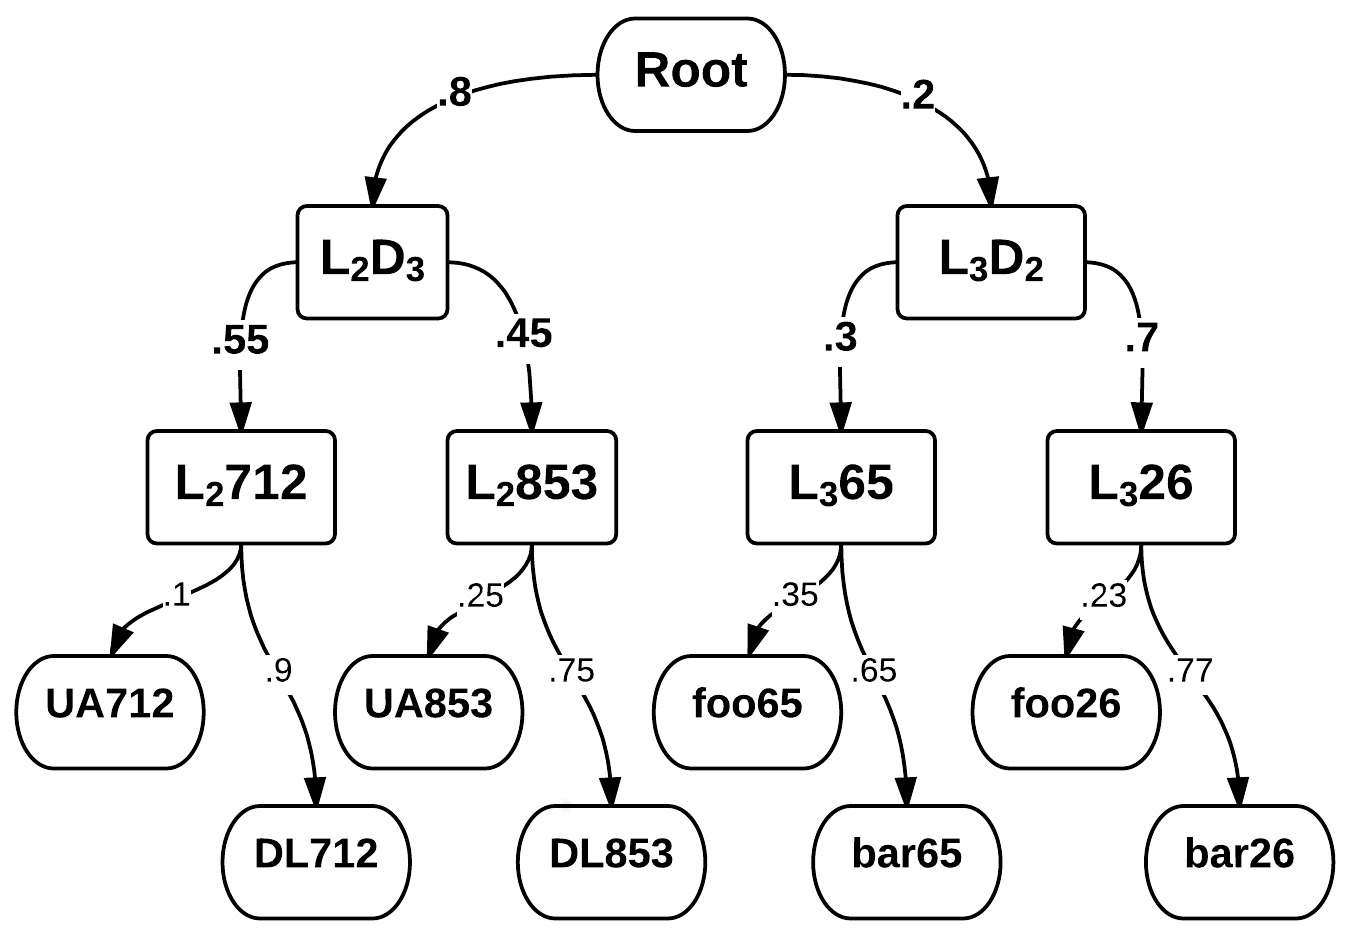
\includegraphics[width=0.45\textwidth]{diag/pcfg.png}
    \end{center}
    \vspace{-10pt}
    \caption{Example PCFG Tree}
    \vspace{-20pt}
    \label{fig:pcfg}
\end{wrapfigure}

\par\quad This enumeration scheme is inspired by natural language processing \cite{pcfg} and provides a more disciplined treatment of password structures. A context-free grammar is formally defined as $\mathcal{G}=(\bm{V}, \bm{\Sigma}, \bm{S}, \bm{P})$, i.e. a tuple of \emph{non-terminals}, \emph{terminals}, \emph{start variable}, and \emph{productions}. While training the model with passwords, probabilities are assigned to each \emph{production} in $\bm{P}$. Eventually, the likelihood of a password can be estimated by its general structure (e.g. six letters followed by one digit) and the values of its components (e.g. the last digit is $3$). Figure \ref{fig:pcfg} on the right shows a small example of PCFG.

\par\quad The initial use of PCFG for password guessability was proposed in \cite{PCFG}, where Weir et al. partitioned password into letter, digit, and special-character substrings. Based on the same model, \cite{againagain} improves guessing efficiency by considering lower- and upper-case letters separately. And, \cite{pcfg-smoothing} furthermore adds smoothing to the learning process by assigning non-zero probability to unobserved password structures. Overall, this scheme gives much better performance than brute-force since it takes into account different likelihood of password structures (e.g. structures like \texttt{Password1} are much more likely than \texttt{a@9Bc4m\#!}) and password contents (e.g. contents like \texttt{superman} are much more likely than \texttt{foqinbgi}) \cite{guessability}.

\subsubsection{Word Mangling Rules}

\begin{wrapfigure}{r}{0.45\textwidth}
    \vspace{-30pt}
    \begin{center}
        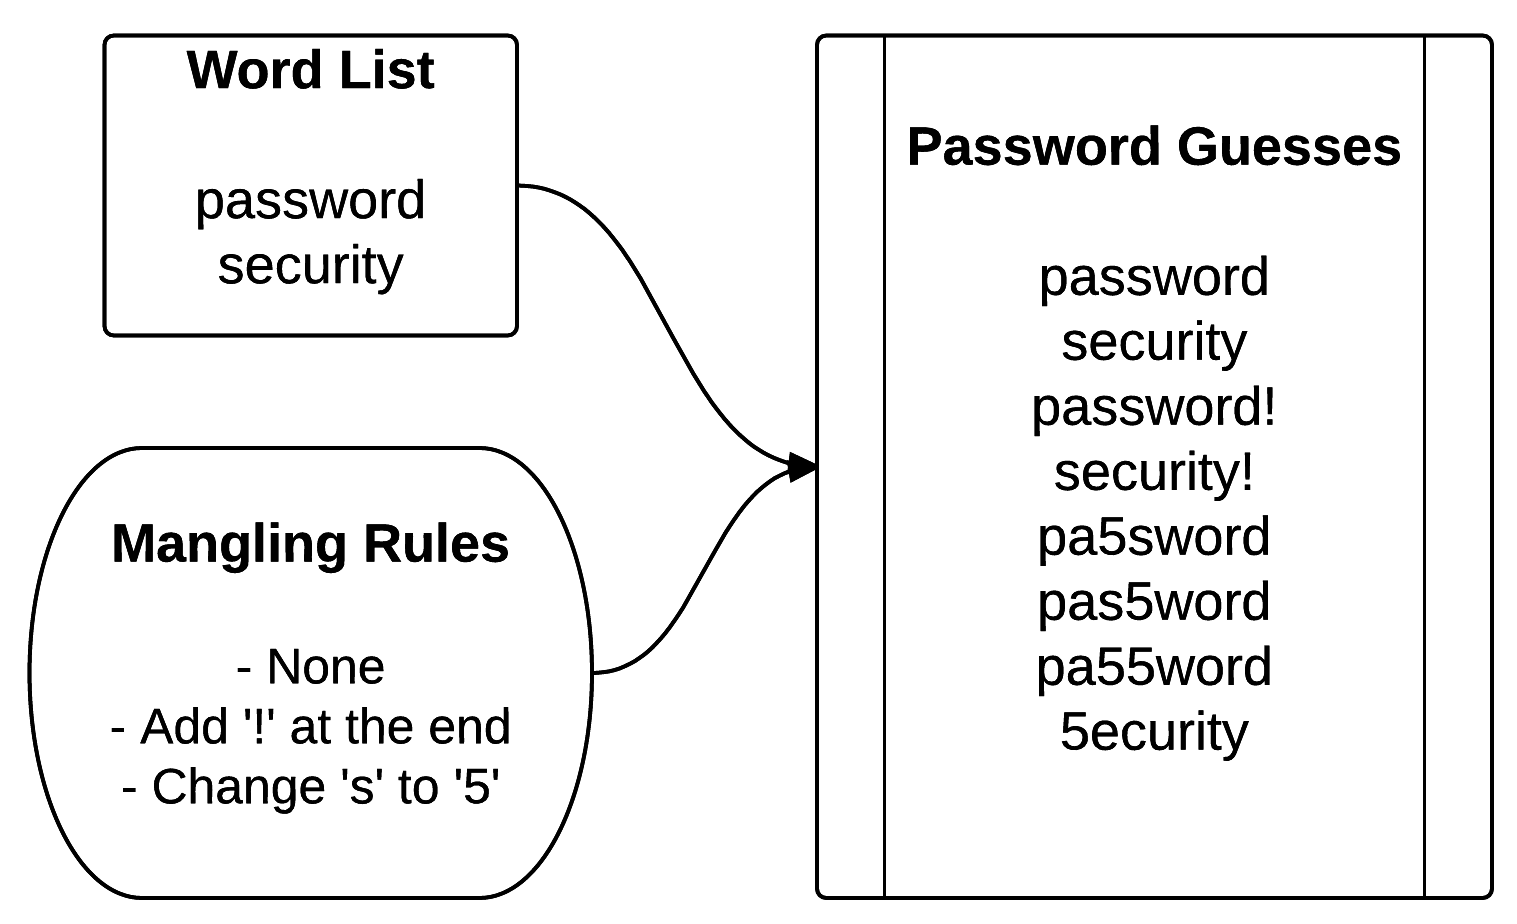
\includegraphics[width=0.45\textwidth]{diag/word_mangling.png}
    \end{center}
    \vspace{-10pt}
    \caption{Sample Word-Mangling Model}
    \vspace{-20pt}
    \label{fig:word-mangling}
\end{wrapfigure}

\par\quad This model has been a favorite of password security professionals thanks to its simplicity and empirical success. Proposed by Morris and Thomson in \cite{history}, the model takes in a \emph{wordlist} and many \emph{word-mangling rules}, and generate password guesses by applying mangling rules on the wordlist provided. A sample run of this approach is shown in Figure \ref{fig:word-mangling}.

\par\quad Popular password cracking utilities including John the Ripper support word-mangling model and provide built-in wordlist and mangling rules \cite{john}. And, \cite{empirical} shows that the default word-mangling model shipped with John the Ripper can be improved by using extra wordlists and customized mangling rules. Overall, the effectiveness of this model relies heavily on its configurations, and fortunately even the default model from John the Ripper has proven to provide favorable results (\cite{pcfg-smoothing}, \cite{mangled2}).

\subsubsection{Markov Model}
\par\quad This stochastic model uses the fact that characters in a password string are \emph{not} independent; more specifically, $k$-grams occur at different probabilities, and a $(k-1)$-gram in a password strongly affects the probability distribution of the next character. For example, \texttt{abcd} is a much more common $4$-gram in passwords than \texttt{abct}, and \texttt{e} is much more likely to occur than \texttt{t} after \texttt{abcd} \footnote{In RockYou password set, $|\texttt{abcd}| = 1173$, $|\texttt{abct}| = 31$, $|\texttt{abcde}| = 704$, and $|\texttt{abcdt}| = 4$.}.

\par\quad Formally speaking, a $k$-gram Markov model (corresponding to a Markov chain of \emph{order} $(k-1)$) can be defined with \emph{initial probabilities} $\Pr[\overline{c_1\cdots c_{k-1}}]$ for every $\overline{c_1\cdots c_{k-1}} \in \Sigma^{k-1}$, and \emph{transition probabilities} $\Pr[c \mid \overline{c_{i}\cdots c_{i+k-2}}]$ for every $\overline{c_{i}\cdots c_{i+k-2}} \in \Sigma^{k-1}$ and $c\in \Sigma$. The probabilities can be estimated by counting the occurrence of $(k-1)$-grams and $k$-grams in the training password set. Figure \ref{fig:markov} shows a simple $3$-gram Markov model populated with transition probabilities.

    \begin{figure}[!htbp]
        \vspace{-30pt}
        \begin{center}
            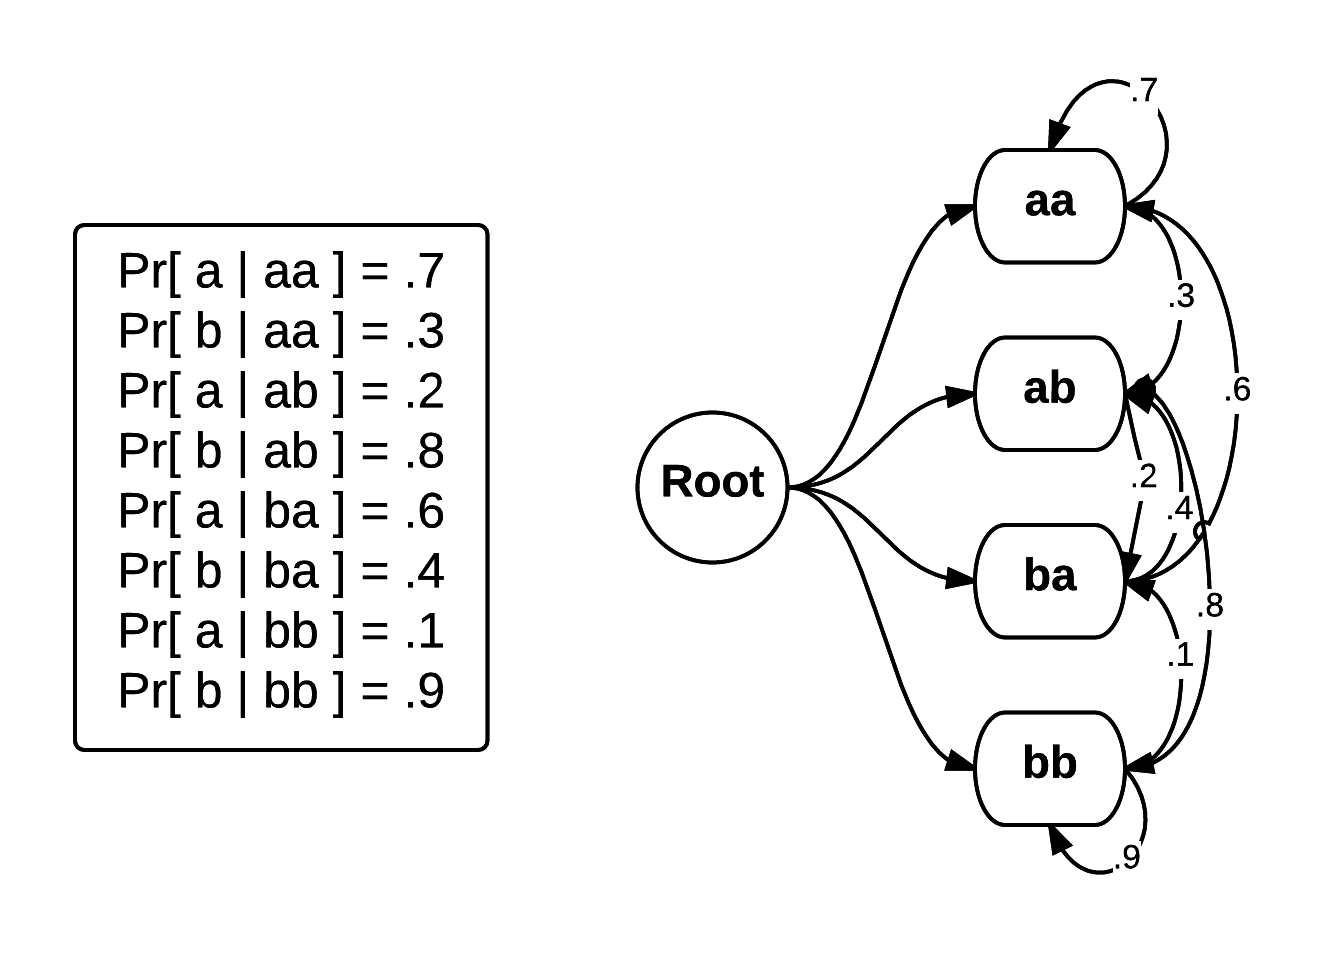
\includegraphics[width=.6\textwidth]{diag/markov.png}
        \end{center}
        \vspace{-20pt}
        \caption{Sample Markov Model with Transition Probabilities}
        \label{fig:markov}
    \end{figure}

\par\quad The use of Markov model in password security was first proposed in \cite{timespace}, where it gave better results than Rainbow attack. Since then, various improvements have been made on the model in various aspects: \cite{adaptive markov} gives an \emph{adaptive meter} for password strength based on Markov model; \cite{empirical} provides an efficient approximation algorithm for counting the number of passwords with probabilities higher than a given threshold by discretization; \cite{omen} proposes a password enumeration scheme that outputs candidates with descending probabilities by using a similar discretization approach; \cite{probframework} and \cite{passmodel} study the use of \emph{layered Markov model}, which generates transition probabilities \emph{per position} in the password.

\par\quad Overall, Markov model has proved more efficient than PCFG in terms of guessing efficiency \cite{guessability}, provided that our model and probabilities are trained carefully. However, this model is more theoretically complicated since it involves a large amount of parameters and states, and it usually takes much longer time per guess than PCFG and word-mangling model. Therefore, it is important to improve the speed of the model to realize its full potential.

\subsubsection{Remarks on Enumeration Heuristics}
\par\quad Previous studies have compared the efficiency of different enumeration strategies for different scenarios. Methods based on brute-force are simple yet inefficient for even moderately large search space; hence, it is often used as a backup option after more efficient methods fail to recover the passwords. As for PCFG, word-mangling model, and Markov model, \cite{guessability} shows that they give similar results overall after proper parameter tuning.

\par\quad Meanwhile, some passwords can be guessed much faster with one heuristic than another. For example, password \texttt{P@ssw0rd!} is easy to guess with mangled wordlist attack by John the Ripper, yet goes beyond cutoff ($10^{14}$ attempts) for PCFG attack \cite{guessability}. This implies that it is important to use multiple approaches simultaneously to crack passwords and measure password security in order to achieve maximal efficiency and accuracy.

\subsection{Measurement of Password Security}
\par\quad Given the password enumeration heuristics discussed above, it is natural to ask the following question: how strong is a password against a heuristic? The common answer is to use \emph{guess number} as the measure, i.e. how many times it takes for a certain enumeration routine to get to a given password. This strategy is widely used in current research (\cite{empirical}, \cite{omen}, \cite{againagain}, \cite{addbang}, and \cite{guessability}), and password guessability services like \cite{cmu-guessability} employ the same philosophy. This measure makes intuitive sense since the larger the guess number, the longer it takes for adversaries to guess a password, and thus the more secure a password tends to be. A major shortcoming of this approach is that calculating the guess number can take a long time, especially for complicated heuristics such as Markov model \cite{probabilistic}.

\par\quad Due to usability concerns, the ``guess number'' approach is usually approximated by \emph{proactive password checkers} empirically. Since the rules are based on length and character composition, the method can sometimes be highly inaccurate, as NIST and Microsoft password meters would classify \texttt{Password1} as ``strong,'' yet it can be easily cracked with PCFG \cite{adaptive markov}.

\par\quad Meanwhile, there are other less direct yet efficient measurements of password security. One candidate is \emph{guessing entropy}, which measures the average number of passwords that need to be guessed before reaching the correct one \cite{adaptive markov}. It is formally defined as follows: for random variable $X$ over finite domain $\mathcal{D}$ with probability distribution $\Pr[X=d_i]=p_i \;\forall i\in[|\mathcal{D}|]$ such that $\langle p_i \rangle_{i\in[|\mathcal{D}|]}$ is non-increasing, $G(X) := \sum_{i=1}^{|\mathcal{D}|}{i \cdot \Pr[X=d_i]}$. This value directly corresponds to the required effort of adversaries in order to crack a password set \cite{entropy}, and is therefore useful for security analysis.

\par\quad There are also efficient metrics designed to measure the security of a \emph{password set}, such as \emph{probability-threshold graph} and \emph{average negative log-likelihood} as proposed in \cite{probabilistic}. Interested readers may refer to the original paper for their usage and limitations.

%%%%%%%%%%%%%%%%%%%%%%%%%%%%%%%%%%%%%%%%%%%%%%%%%%%%%%%%%%%%%%%%%%%%
%%%%%%%%%%%%%%%%%%%%%%%%%%%%%%%%%%%%%%%%%%%%%%%%%%%%%%%%%%%%%%%%%%%%
\section{Markov-based Guess Number Calculator}
\par\quad In this section, we will first cover some technical background relevant to passwords and probability. Then, we will analyze our training data, describe our Markov model, and propose our algorithm for creating a look-up table based on the Markov model. Eventually, given a password that the look-up table covers, our method can calculate its guess number very efficiently.

\subsection{Technical Background}
\par\quad Before presenting our methodology, we introduce readers to terminologies and notations relevant to probability and password security that will be used for the rest of the report. Some definitions are inspired by previous studies, including \cite{adaptive markov}, \cite{omen}, \cite{probabilistic}, and \cite{timespace}.

\vskip 5px
\begin{defn}
    A \emph{password} $s$ is a sequence of $n\in\mathbb{N}^*$ characters of the form $s=\langle s_1s_2\cdots s_n\rangle$ from an alphabet $\Sigma$, such that $s_j\in\Sigma$ for $j=1,2, \cdots, n$.
\end{defn}

\vskip 5px
\begin{defn}
    A \emph{password probability model} (or \emph{password model}) is a function $p : \Gamma \to [0,1]$ that assigns a probability to each password in password universe $\Gamma$, such that $\sum_{s\in\Gamma}{p(s)}=1$.
\end{defn}

\vskip 5px
\begin{defn}
    A \emph{$k$-gram Markov model} is a probabilistic model that models the probability of the next character in a password based on previous $(k-1)$ characters. With such model, given a password $s=\langle s_1s_2\cdots s_n\rangle$ with $n \geq k-1$, its probability measure is:
        \begin{equation} \label{eq:markov}
            p(s) := \Pr[\overline{s_1\cdots s_{k-1}}] \cdot \left(\prod_{i=k}^{n}{\Pr[s_i \mid \overline{s_{i-k+1}\cdots s_{i-1}}]}\right) \cdot \Pr[\bot \mid \overline{s_{n-k+2}\cdots s_{n}}].
        \end{equation}
\end{defn}
\begin{remark}
    In Formula (\ref{eq:markov}) above, the first term corresponds to \emph{starting probability} of the prefix with length $(k-1)$; the middle term corresponds to \emph{transition probabilities} for intermediate characters; the last term is \emph{end-symbol normalization factor} \cite{probabilistic}, where $\bot$ is specially reserved for end-of-password.
\end{remark}

\vskip 5px
\begin{defn}\label{def:nll}
    The \emph{negative log-likelihood} (NLL) of a password $s=\langle s_1s_2\cdots s_n\rangle$ in a $k$-gram Markov model is defined as:
    {\footnotesize
    \begin{equation}
        \ell(s) := -\log(p(s)) = -\log\Pr[\overline{s_1\cdots s_{k-1}}] - \left(\sum_{i=k}^{n}{\log\Pr[s_i \mid \overline{s_{i-k+1}\cdots s_{i-1}}]}\right) - \log\Pr[\bot \mid \overline{s_{n-k+2}\cdots s_{n}}]
    \end{equation}
    }
\end{defn}
\begin{remark}
    The benefit of NLL includes transforming probability multiplication to log-likelihood addition, which makes calculation and optimization more convenient.
\end{remark}


\subsection{Training Data Analysis}     \label{sect:data-analysis}
\par\quad Our training dataset contains leaked passwords from RockYou and Unix English dictionary \footnote{On Ubuntu, the dictionary is a newline-delimited file located at \texttt{/usr/share/dict/words}.}. We believe our use of leaked password for the study is justifiable because the passwords are already available to public, and because the passwords are not associated with usernames. Also, we are incorporating natural-language dictionary in our training since real-world passwords are often derived from dictionary words. Moreover, including the dictionary allows us to not only analyze the strength of existing passwords but also to predict that of potential future passwords.

\par\quad Overall, the RockYou dataset contains 32.6 million passwords (with 14.3 million unique entries), and the Unix dictionary contains 99,171 entries. To understand the composition of our training set, we studied the following statistics:

\begin{itemize}
    \item Character composition: We wish to study the common and uncommon characters in our dataset in order to reduce the size of the alphabet (more on this later). Out of all entries in the original dataset, more than 99.9\% contain only characters with ASCII values in the range $[32,126]$, which correspond to regular, printable characters. A more detailed character distribution is in Figure \ref{fig:chardistribution} below. We noticed that the majority of characters are lowercase and digits (96.1\%), and there are occasionally uppercase letters (3.2\%) and rarely special characters (0.7\%). 
    
    \begin{figure}[!htbp]
        \begin{center}
            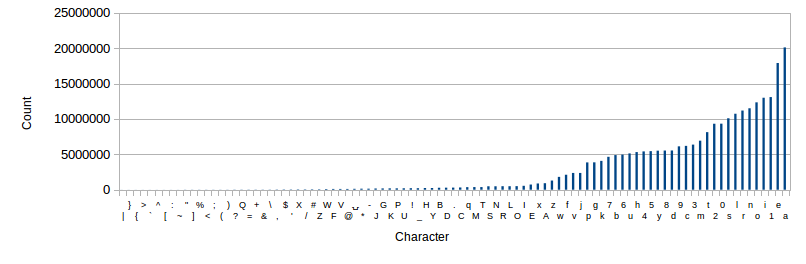
\includegraphics[width=\textwidth]{diag/chardistribution.png}
        \end{center}
        \vspace{-15pt}
        \caption{Character Composition of Training Set}
        \label{fig:chardistribution}
    \end{figure}
    
    \item Password patterns: To understand the common patterns of dataset, we matched it against several regular expressions (some are inspired by \cite{empirical}), and the results are in Table \ref{table:patterns}. We noticed that the majority ($96.2\%$) of entries only contain letters and digits. We then considered adding several extra characters in our alphabet to improve coverage, and it turns out that adding the most common special characters gives efficient return (up to $99.3\%$ matching).
    
    \begin{table}[!htbp]
        \vspace{-5pt}
        \begin{center}
            \begin{tabular}{|c|c|c|c|c|}
                \hline
                RegEx:                                  & Example:                      & Match Count:  & Match Percentage:     \\ \hline \hline
                \texttt{\string^[a-z0-9]+\$}            & \texttt{a1b2c3}               & 29659726      & 90.7\%        \\ \hline
                \texttt{\string^[a-zA-Z0-9]+\$}         & \texttt{a1B2c3}               & 31434981      & 96.2\%        \\ \hline
                \texttt{\string^[\string^a-z0-9]+\$}    &\texttt{A@WG|Y)}               & 523111        & 1.60\%        \\ \hline
                \texttt{\string^[\string^a-zA-Z0-9]+\$} & \texttt{;|>+\}\$!}            & 5040          & 0.015\%       \\ \hline \hline
                
                \texttt{\string^[a-zA-Z0-9\textbackslash.\_!-\textbackslash*]+\$}       & \texttt{-}    & 32151927      & 98.4\%        \\ \hline
                \texttt{\string^[a-zA-Z0-9\textbackslash.\_!-\textbackslash* @\#/']+\$} & \texttt{-}    &  32456273     & 99.3\%        \\ \hline
            \end{tabular}
        \end{center}
        \vspace{-5pt}
        \caption{String Patterns in Training Set ($N = 32,684,277$)}
        \vspace{-15pt}
        \label{table:patterns}
    \end{table}
\end{itemize}

\par\quad The observations above show that alpha-numeric characters and some high-frequency special characters dominate our training set, and this will be an important insight when we decide on the alphabet size for our Markov model.

\subsection{$k$-gram Markov Model Builder with Smoothing}       \label{sect:smoothing}
\par\quad Given the training data, our first step is to gather necessary statistics and build a $k$-gram Markov model. To calculate the probabilities of the model, we first run through the training data and keep track of initial $(k-1)$-gram counts, $k$-gram counts, and terminal $(k-1)$-gram counts. The routine is described in Algorithm \ref{algo:statgen}.

\begin{algorithm}[!htbp]
\renewcommand\footnoterule{}
    \caption{Statistics Generation Routine (\texttt{statgen})}
    \label{algo:statgen}
    \begin{algorithmic}
        \Require{$k$, input dataset $\mathcal{D}$}
        \Ensure{Mappings StartCount, MidCount, EndCount}
        
        \State
        \State StartCount, MidCount, EndCount $\gets \{\vec{0}\}$;       \Comment{Default value of mappings set to zero}
        \State
        \Function{train\_markov}{word}
            \State $n \gets $ len(word);
            \State StartCount[ word[:(k-1)] ]++;
            \State EndCount[ word[-(k-1):] ]++;
            \For{start = 0 to n-k}
                \State MidCount[ word[start:start + k] ]++;
            \EndFor
            \State \Return
        \EndFunction
        
        \State
        \ForAll{word $\in \mathcal{D}$}
            \State \Call{train\_markov}{word};
        \EndFor
        \State Output StartCount, MidCount, EndCount;
    \end{algorithmic}    
\end{algorithm}

\par\quad For the higher-order Markov model we are constructing, sparseness can be an issue since our training dataset is limited compared to parameter size. For example, assuming an alphabet of size $62$ (i.e. alpha-numeric characters) and $k=5$ (as adopted by \cite{omen} and \cite{probabilistic}), there are $62^{5-1} \approx 14.8$ million potential starting $4$-grams, yet our training set only contains $32.7$ million entries. To offset the sparseness, our top candidate for smoothing algorithm is \emph{additive smoothing}, as it is an intuitive routine commonly used in Machine Learning. It essentially adds a pseudocount $\delta>0$ to each of the starting or ending $(k-1)$ gram and conditional character count, such that even if a sample does not appear in the dataset, we assign it a \emph{non-zero yet small} probability in our model. In Algorithm \ref{algo:probgen} below, we present the pseudocode for our probability generation routine with support of additive smoothing.

\begin{algorithm}[!htbp]
    \caption{Probability Calculation with Additive Smoothing (\texttt{probgen})}
    \label{algo:probgen}
    \begin{algorithmic}
        \Require{$k$, $\delta$, $\Sigma$; StartCount, MidCount, EndCount from \texttt{statgen} (Algorithm \ref{algo:statgen})}
        \Ensure{Mappings StartProb, MidProb, EndProb}

        \State
        \State StartProb, MidProb, EndProb $\gets \{\}$;
        \State
        \State StartCountTotal $\gets \sum_{w\in\Sigma^{k-1}}{\text{StartCount[w]}}$;
        \State EndCountTotal $\gets \sum_{w\in\Sigma^{k-1}}{\text{EndCount[w]}}$;
        \ForAll{word $\in \Sigma^{k-1}$}
            \State StartProb[word] $\gets \dfrac{\text{StartCount[word]} + \delta}{\text{StartCountTotal} + \delta \cdot |\Sigma|^{k-1}}$;
            \State EndProb[word] $\gets \dfrac{\text{EndCount[word]} + \delta}{\text{EndCountTotal} + \delta \cdot |\Sigma|^{k-1}}$;
        \EndFor
        
        \State
        \ForAll{prefix $\in \Sigma^{k-1}$}
            \State PrefixCount $\gets \sum_{c\in\Sigma}{\text{MidCount[$\overline{\text{prefix}\; c}$]}}$;
            \ForAll{next $\in \Sigma$}
                \State MidProb[$\overline{\text{prefix}\; c}$] $\gets \dfrac{\text{MidCount[$\overline{\text{prefix}\; c}$]} + \delta}{\text{PrefixCount} + \delta\cdot |\Sigma|}$; 
            \EndFor
        \EndFor
        
        \State Output updated StartProb, MidProb, EndProb;
    \end{algorithmic}
\end{algorithm}

\subsection{Probability Discretization}
\par\quad In order to support efficient enumeration of passwords in decreasing probability, we use the similar \emph{probability discretization} approach as in Ordered Markov Enumerator proposed by D\"{u}rmuth et al \cite{omen}. The approach discretizes probability values into integer values between $0$ and $\eta > 0$ (inclusive) by using the following formula:
    \begin{equation}
        lvl(p) = -\text{round}(\log(c_1 \cdot p + c_2)).
    \end{equation}
Note that $c_1$ and $c_2$ are \emph{scaling} and \emph{shifting constants} in order to make all ``levels'' stay between $0$ (for highest $p$) and $\eta$ (for lowest $p$).

\par\quad To calculate the values of $c_1$ and $c_2$ for each of StartProb, MidProb, and EndProb probability set in Algorithm \ref{algo:probgen}, assume the maximal probability value in the mapping is $p_{\max}$. Then, we can simply solve for $c_1$ and $c_2$ from the following system:
    \begin{equation}
        \begin{cases}
            -\log(c_2) = \eta\\
            \log(c_1 p_{\max} + c_2) = 0
        \end{cases},
    \end{equation}
which solves to $(c_1, c_2) = \left(\frac{1-\exp(-\eta)}{p_{\max}}, \exp(-\eta)\right)$.

\par\quad With probability discretization, we may approximate the likelihood of a password by adding up the probability levels just like adding up the individual log-probabilities in the definition of \emph{negative log-likelihood} in Definition \ref{def:nll}. This will make our enumeration routine mentioned below more efficient.

\subsection{Markov Model Enumeration} \label{sect:enumeration}
\par\quad Before we present our look-up table in the next section, it is sensible to understand the state-of-the-art Markov model enumeration technique discussed in this section, since our final goal is to calculate the guess number based on this enumeration model efficiently.

\par\quad Given the ``level'' data from previous steps, we wish to enumerate passwords such that the total levels of them roughly increase over time -- by doing so, we indeed go over the more likely passwords first. In order to do so, we will reverse-engineer how we calculate the \emph{total level} of a password by splitting the the total into a list of levels that sum up to it, and each of them would represent \emph{starting level}, \emph{transition level}, and \emph{ending level}, depending on its location in the list (similar approach is used in \cite{omen}).

\par\quad As for the length of our list, note that for a password with length $n$, there should be \emph{one} starting level, $(n-k)$ intermediate levels, and eventually one ending level. Thus, the length of the list we are generating is $(n-k+2)$, where each element is betewen $0$ and $\eta$ (inclusive), and we wish to make the sum of the list $\ell$, i.e. the level we are considering.

\par\quad Meanwhile, one concern is that the lengths of our passwords are not fixed. To consider multiple lengths simultaneously, we again follow a similar approach to \cite{omen}; however, since we do not have a notion of \emph{success probability} in our case, we need to use something different -- given a password with length $\ell$ and total level $lvl$, define the \emph{complexity} of a password as: $\texttt{complexity} = \ell + \beta\cdot lvl$, i.e. a linear combination of the length and total level. While we are enumerating the passwords, we pick the (length,level)-pairs ascendingly by their \emph{complexity measure}. This allows us to shift to likely, longer passwords instead of staying at shorter yet unlikely passwords\footnote{An alternative approach is to analyze the training dataset and discretize ``length probabilities.'' Then, the \emph{complexity measure} is based on the discretized length probabilities instead of length itself. However, for our use case, the original model suffices.} (e.g. password \texttt{password} is much more likely than \texttt{pqciun} even though it is longer).
\par\quad Based on this approach, for each (length,level)-pair we enumerate all matching options by running an algorithm similar to depth-first search, and this continues until we find our target password or hit the ``maximal guess count threshold $T$.'' Overall, the enumeration algorithm is presented in Algorithm \ref{algo:passenum} below.

\begin{algorithm}[!htbp]
    \caption{Password Enumerator (\texttt{passenum})}
    \label{algo:passenum}
    \begin{algorithmic}
        \Require{$k$, $\beta$, $\Sigma$; trial threshold $T$; input password $s_0$; probability levels \emph{StartLevel}, \emph{MidLevel}, \emph{EndLevel}}
        \Ensure{Estimated guess number $N$}
        \State
        \State\comment{// Explore passwords with length \texttt{len} and level \texttt{lvl}}
        \Function{enum\_pass}{len, lvl, so\_far = \texttt{``''}, remaining\_lvl = level}
            \If{len(so\_far) == len}      \Comment{Base Case I: All chars chosen; verify level}
                \State attempt\_count++;
                \If{attempt\_count $\geq T$}
                    \State\Return{\texttt{BEYOND\_THRESHOLD}};
                \EndIf
                \State\Return{remaining\_lvl == 0 ? \texttt{SUCCESS} : \texttt{NOT_SUCCESS}};
            \Else                       \Comment{Inductive Case: Add char the recurse}
                \For{next\_lvl = 0 to $\min(\eta, \text{remaining\_lvl})$}
                    \For{next\_char \textbf{in} MidLevel[ so\_far[-(k-1):] ] [next\_lvl]}
                        \If{\Call{ENUM\_PASS}{len, lvl, so\_far + next\_char, remaining_lvl - next\_lvl} == \texttt{SUCCESS}}
                            \State\Return{\texttt{SUCCESS}};
                        \ElsIf{\_\_ == \texttt{BEYOND\_THRESHOLD}}
                            \State\Return{\texttt{BEYOND\_THRESHOLD}};
                        \EndIf
                    \EndFor
                \EndFor
                \State\Return \texttt{NOT_SUCCESS};
            \EndIf
        \EndFunction        

        \State
        \State\comment{// Main guessing routine -- keep looping until password guessed}
        \State attempt\_count $\gets 0$;
        \While{\textbf{true}}
            \State (length, level) $\gets$ pending pair with minimal $(\text{length} + \beta\cdot\text{level})$;
            \State result $\gets$ enum\_pass(length, level)\;
            \If{result == \texttt{SUCCESS}}
                \Return attempt\_count;
            \ElsIf{result == \texttt{BEYOND\_THRESHOLD}}
                \textbf{break};
            \EndIf
        \EndWhile
        \State\Return{\texttt{Beyond threshold!}}
    \end{algorithmic}
\end{algorithm}

\subsection{Password Guessability Look-Up Table} \label{sect:lookup}
\par\quad This component is the core of our contribution. From the enumeration routine described in the previous section, it is important to learn the following:
\begin{enumerate}
    \item We consider passwords with the same (length, level) values together as an independent segment, i.e. passwords with different (length, level) property are \emph{never} mixed together. Also, the (length, level) pairs themselves constitute a \emph{total ordering} by the value of $(\text{length} + \beta\cdot\text{level})$ as proposed in the previous section;
    \item If we fix our input statistics and a (length, level)-pair, the order in which we enumerate the passwords does \emph{not} change since we follow a deterministic depth-first search order in our dictionaries \emph{StartLevel}, \emph{MidLevel}, and \emph{EndLevel}.
    \item Across different runs of password guessing, essentially the same DFS process is run multiple times, which is totally wasteful. 
\end{enumerate}

\par\quad Given the observations above, we build our look-up table as follows: for each (length, level)-pair, run the \texttt{enum\_pass} routine above, while \emph{taking note of every $m$ guesses we make}. This would give us a list of \emph{checkpoints} for each (length, level)-pair. In Figure \ref{fig:checkpoint} below, we show a small example of \emph{checkpointing} with $\text{length}=2$, $\text{level}=3$, and $m=3$.

    \begin{figure}[!htbp]
        \vspace{-15pt}
        \begin{center}
            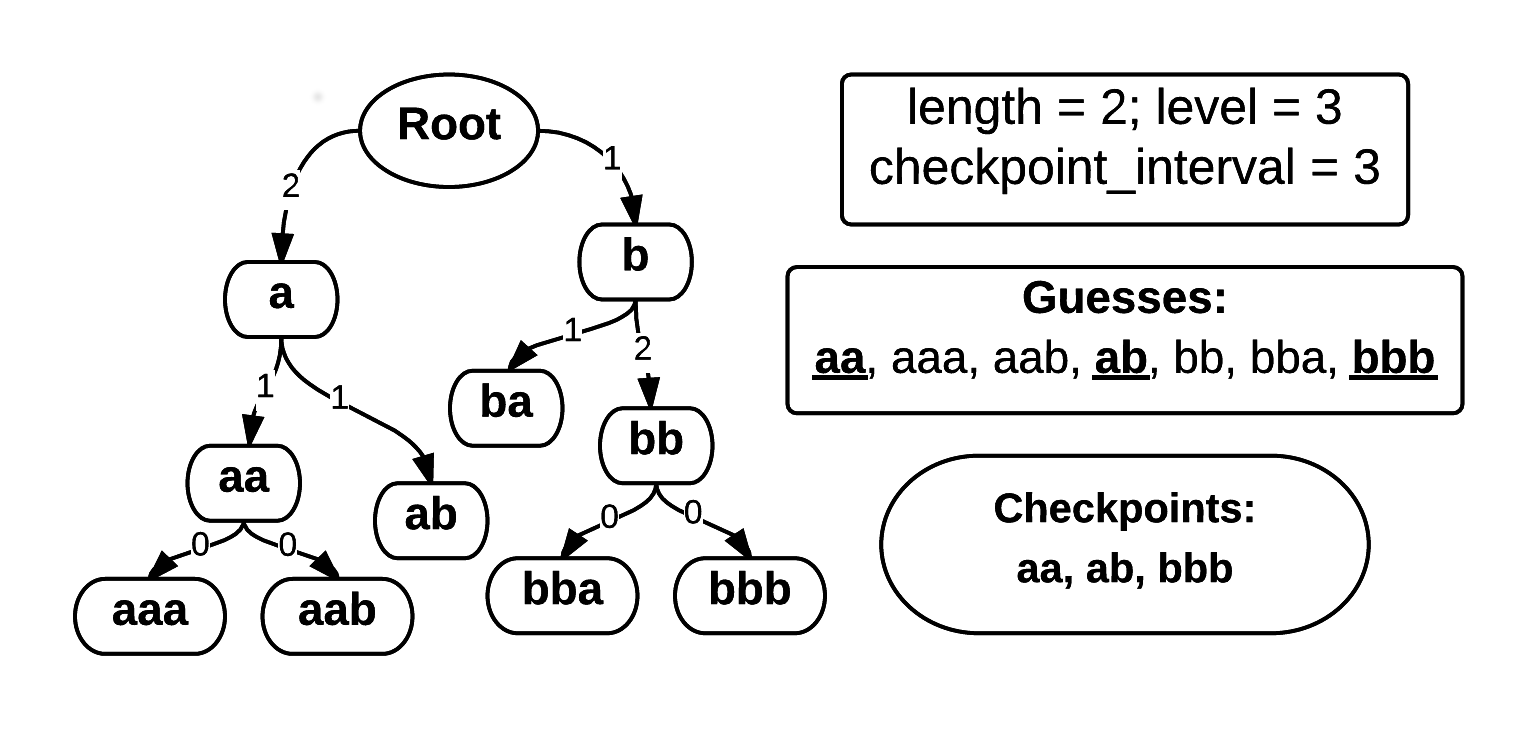
\includegraphics[width=.8\textwidth]{diag/checkpoint.png}
        \end{center}
        \vspace{-15pt}
        \caption{Example of Checkpointing}
         \vspace{-5pt}
        \label{fig:checkpoint}
    \end{figure}

\par\quad Once we have built the checkpoints for each (length, level)-pair in a pre-defined range, calculating the guess number of a password is much more efficient, as shown in Algorithm \ref{algo:newpassenum} below. We can first calculate the target (length,level)-pair, then skip over \emph{all prior cases}. Even inside the case of (length, level) itself, we may skip over cases in which the choice at any point would happen before to our latest checkpoint. Overall, our new algorithm offers a tremendous amount of trimming, and as shown in Section \ref{sect:results}, the time-saving effect can be huge.

\begin{algorithm}[!htbp]
    \caption{\emph{New} Password Enumerator (\texttt{new-passenum})}
    \label{algo:newpassenum}
    \begin{algorithmic}
        \Require{$k$, $\beta$, $\Sigma$; trial threshold $T$; input password $s_0$; probability levels \emph{StartLevel}, \emph{MidLevel}, \emph{EndLevel}; \emph{Checkpoints} $\mathcal{C}_{\text{len, lvl}}$.}
        \Ensure{Estimated guess number $N$}
        \State
        \State\comment{// Explore passwords with length \texttt{len} and level \texttt{lvl}}, \emph{subject to lower_bound}
        \Function{enum\_pass}{len, lvl, so\_far = \texttt{``''}, remaining\_lvl = level, \textbf{lower\_bound}}
            \If{len(so\_far) == len}      \Comment{Base Case I: All chars chosen; verify level}
                \State attempt\_count++;
                \State\Return{remaining\_lvl == 0 ? \texttt{SUCCESS} : \texttt{NOT_SUCCESS}};
            \Else                       \Comment{Inductive Case: Add char the recurse}
                \For{next\_lvl = 0 to $\min(\textbf{lower\_bound[len(so\_far)]}, \text{remaining\_lvl})$}       \Comment{Skip lower cases!}
                    \For{next\_char \textbf{in} MidLevel[ so\_far[-(k-1):] ] [next\_lvl]}
                        \If{\Call{ENUM\_PASS}{len, lvl, so\_far + next\_char, remaining_lvl - next\_lvl} == \texttt{SUCCESS}}
                            \State\Return{\texttt{SUCCESS}};
                        \EndIf
                    \EndFor
                \EndFor
                \State\Return \texttt{NOT_SUCCESS};
            \EndIf
        \EndFunction        

        \State
        \State (length, level) $\gets$ $($len($s_0$), level($s_0$)$)$;  \Comment{Fast calculation given level indeces}
        \If {(length, level) beyond limit}
            \State\textbf{exit}(\texttt{BEYOND\_THRESHOLD});
        \EndIf
        \State\comment{// Skipping all prior cases}
        \State attempt\_count $\gets 0$;
        \For{(prev\_len, prev\_lvl) that happen before (length, level)}
            \State attempt\_count += $\mathcal{C}_{\text{prev\_len, prev\_lvl}}\text{.count}$;  \Comment{Skip the entire case!}
        \EndFor
        \State\comment{// Calculate the guess number in current case}
        \State latest\_checkpoint $\gets$ binary\_search in $\mathcal{C}_{\text{length, level}}$ for last checkpoint prior to $s_0$
        \State \Call{ENUM\_PASS}{(length, level, \textbf{lower\_bound=latest\_checkpoint}}      \Comment{Skip attempts below latest checkpoint}
        \State\Return{attempt\_count};
    \end{algorithmic}
\end{algorithm}

\subsection{Parameter-Tuning}
\par\quad Previous studies (e.g. \cite{guessability}) have shown that parameter-tuning is as important as choosing a suitable model. After presenting our algorithm above, we will now discuss our decisions in tuning its parameters. Especially, we will discuss how we decided on several key parameters in the model from a theoretical standpoint.

\subsubsection{Alphabet Size}
\par\quad It is a well-supported fact that larger alphabet costs more computational and storage resources in exchange for higher password coverage and hence guess rate (\cite{adaptive markov}, \cite{empirical}, \cite{omen}). In order to decide on an appropriate alphabet size to use, we surveyed many relevant literatures and found that the most common approaches include: keep top $m (\geq 50)$ characters by frequency, keep alphanumeric characters, keep alphanumeric characters plus $m (\leq 20)$ most popular special characters.

\par\quad Based on the observations in Section \ref{sect:data-analysis}, we noted that alphanumeric characters cover $96.2\%$ passwords of our training dataset, and that top-$50$ characters account for more than $98.6\%$ of characters in the training set. However, we did not use the ``most popular $m$-chars'' approach since it is inherently unfair -- for example, even when $m=60$, characters like $\textvisiblespace$ and $F$ are not chosen, which are common components of most human languages. As for the ``alphanumeric + special-char'' approach, we did not choose it since the average marginal return of the additional characters is too low -- for example, for $k=4$, the number of \emph{transition probabilities} we need to keep track of nearly doubles due to the additional characters, yet the password coverage increases only by $3\%$. Nonetheless, we belive this comprehensive alphabet would be suitable for enterprise or research users, who have more computational resources for the algorithm.

\par\quad Eventually, we decided on using \emph{alphanumeric characters} as our alphabet, which consists of \emph{62} characters.

\subsubsection{$k$-gram Size}
\par\quad $k$-gram size determines since how far back in a password the next character depends on. Overall, a higher value of $k$ would provide better accuracy since a longer history is considered, \emph{provided that sufficient training data is available}. On the other hand, a larger $k$-gram size can not only increase the number of our parameters exponentially (i.e. $\mathcal{O}(|\Sigma|^k)$), but might also cause a potential problem of \emph{sparsity}, which we partially addressed in Section \ref{sect:smoothing} with smoothing. As an example, when the value of $k$ goes beyond $5$, $|\Sigma|^k \gtrsim 10^9$, while it is practically impossible to gain that much training data.

\par\quad For our Markov model in this study, we choose to use $k=3$ such that sparseness would not be an issue for us, and that the algorithm can run fast enough to generate enough checkpoints for our testing. Nonetheless, for professional settings, previous studies have shown that a slightly larger $k$-value, i.e. $k=4$ or $5$ would offer a higher rate of success (\cite{omen}, \cite{probabilistic}).

\subsubsection{Maximal Probability Level ($\eta$-size)}
\par\quad The value of $\eta$ determines the amount of discretization of probability values, and \cite{omen} analyzed its effect briefly -- when $\eta$ is low, the probabilities are bucketed more coarsely, thereby giving a shorter run-time yet weaker ``orderedness'', and vice versa. We decided to pick $\eta=10$ just like in \cite{omen} to achieve a balance between run-time and orderedness.

\subsubsection{Checkpoint Interval ($\mathcal{I}$)}
\par\quad This is the only parameter specific to our algorithm. As shown in Algorithm \ref{algo:newpassenum}, our enumeration model can essentially ``jump'' to the latest checkpoint and continue its search from there. In order to locate the checkpoint, the binary search gives a complexity of order $\mathcal{O}(\log \frac{N}{\mathcal{I}}) = \mathcal{O}(-\log\mathcal{I})$, where $N$ denotes the number of password guesses for a certain (length,level)-pair. From the checkpoint, our algorithm will make at most $\mathcal{O}(\mathcal{I})$ guess attempts. Thus, in total the work complexity for calculating a new guess number is $\mathcal{O}(\mathcal{I})$.

\par\quad Meanwhile, the storage required for checkpoints is inversely proportional to $\mathcal{I}$ since we record one password guess out of every $\mathcal{I}$. As a rough estimation, assume that passwords in the checkpoints have length $11$ on average and are delimited by new-lines. In order to store the checkpoints for the first $10^{14}$ guess, the total storage is $\frac{10^{14}}{\mathcal{I}} \cdot (11 + 1) \text{ byte} = \frac{1200}{\mathcal{I}} \text{ TB}$. Thus, for professional environments, even $\mathcal{I}=1,000$ is reasonable since the algorithm uses $1.2$ TB of storage and only goes through $1000$ password guesses \footnote{For huge dataset like this, I/O throughput would be more important than the efficiency of algorithm itself.}.

\par\quad In our study, we chose to use $\mathcal{I}=10,000$ because we only have limited-size, consumer-grade HDD instead of huge SSD's available in research environments. Also, $\mathcal{I}=10,000$ would still give us satisfactory calculation speed.

\subsection{Implementation Details}
\par\quad In this section, we will discuss how we implemented our algorithm, with special focus on the unintuitive indexing and mapping optimizations we used. Overall, we decided to use Python 2 as our programming language since it is suitable for handling data and is the most familiar to us. While the performance of Python raises a potential concern, we adopted Pypy, an alternative implementation of Python that uses Just-in-Time compilation, which typically offers at least 5x speedup \footnote{Benchmark data available at: \url{http://speed.pypy.org/}.} compared to the default implementation (i.e. \texttt{CPython}).

\par\quad Our code consists of three modules: \emph{training module}, \emph{enumeration module}, and \emph{calculation module}. Inside \emph{training module}, the first step (\texttt{statgen.py}) digests input data and outputs Markov probabilities as JSON files at \texttt{./data/probs/*\_*\_*.json}, which will be used for probability discretization. Then, the second step discretizes probabilities and organizes them into indeces for convenient retrieval by \emph{enumeration step} later. As shown in the algorithms above, since we often iterate over ``$(k-1)$-gram prefixes/suffixes with certain probability level'' and ``next-characters with certain probability level after prior $(k-1)$-gram,'' we store the probability levels as the following mappings in JSON format:
\begin{gather*}
\text{StartLevel} / \text{EndLevel} := \{ \text{probability\_level} \mapsto [\text{prefixes / suffixes}] \}                 \\
\text{MidLevel} := \{ \texttt{$(k-1)$-gram} \mapsto \{ \text{probability\_level} \mapsto [\text{next\_chars}]\} \}
\end{gather*}
Overall, Figure \ref{fig:components-training} gives a visual representation of the training module.

    \begin{figure}[!htbp]
        \begin{center}
            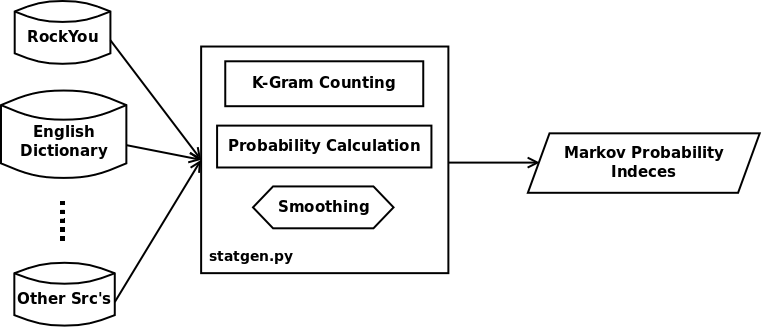
\includegraphics[width=.65\textwidth]{diag/components-training.png}
        \end{center}
        \vspace{-15pt}
        \caption{Components of Training Module}
        \label{fig:components-training}
    \end{figure}

\par\quad As for \emph{enumeration module} (\texttt{checkpoint.py}), we implemented the depth-first search in Algorithm \ref{algo:newpassenum} with efficient trimming: for example, if ``max\_level $*$ remaining\_chars $<$ remaining\_lvl'', we know that the current prefix will not be able to construct any valid passwords, so we safely trim the case. Also, since the different DFS instances are independent, we were able to run multiple of them in parallel by using \texttt{xrargs} in \texttt{bash}, thereby achieving linear speedup.

\par\quad At last, in \emph{calculation module} (\texttt{guess.py}), we need to perform binary search on the checkpoints based on the order of guessing. In order to formalize \emph{DFS-ordering} in our case, we \emph{decompose} a password $s$ with length $n$ into a sequence of triplets as follows:
\begin{equation}
    \texttt{decompose}(s) := \langle(\text{level}_i, \text{index}_i, \text{content}_i)\rangle_{i=0}^{n-k+1},
\end{equation}
such that \emph{$\text{level}_0$} is the level of the $(k-1)$-prefix, \emph{$\text{index}_0$} is the index of the prefix in the list of prefixes with level $\text{level}_0$, and \emph{$\text{content}_0$} is the actual string of the $(k-1)$-prefix. Similar definition follows for \emph{$\text{level}_i$}, \emph{$\text{index}_i$}, and \emph{$\text{content}_i$} with $i>0$. With this definition, we can deduce the ordering of two passwords by comparing the two sequences element-by-element. Following is a simple example with $k=5$, where the level and index values are hypothetical:
\begin{gather*}
    \texttt{s1} = \text{``passwd''};\; \texttt{decompose}(s1) = \langle(3, {\bf 186}, \text{``pass''}), (2, 8, \text{``w''}), (5, 2, \text{``d''})\rangle;    \\
    \texttt{s2} = \text{``p23456''};\; \texttt{decompose}(s2) = \langle(3, {\bf 252}, \text{``p234''}), (1, 2, \text{``5''}), (0, 3, \text{``6''})\rangle;
\end{gather*}
Based on the decompositions above, we can deduce that password ``passwd'' is guessed \emph{before} ``p23456'' since $252 > 186$ in the second entry of the first triplet.

\par\quad Overall, the scripts \texttt{statgen.py} and \texttt{discretization.py} are to be executed once for the entire dataset in order to calculate the discrete probabilities. Then, \texttt{checkpoint.py} instances are run in parallel for different combinations of length and total level, the range of which depends on resources available and use case of the algorithm. Eventually, \texttt{guess.py} is the user-facing script that calculates the guess number for any given password in range. Selected source code from the scripts are included in Appendices B-D.

%%%%%%%%%%%%%%%%%%%%%%%%%%%%%%%%%%%%%%%%%%%%%%%%%%%%%%%%%%%%%%%%%%%%
%%%%%%%%%%%%%%%%%%%%%%%%%%%%%%%%%%%%%%%%%%%%%%%%%%%%%%%%%%%%%%%%%%%%
\section{Results \& Evaluation} \label{sect:results}
\par\quad In this section, we present the result of our implementation. We first specify the model parameters and our environment for running the code suite. Then, we break down to individual modules and analyze their benchmarks. Eventually, we verify that our password model is reasonable by feeding it various passwords and compare the results with common wisdoms about password security.

\subsection{Model Parameters \& System Specification}
\par\quad As chosen in previous sections, following are the parameters used in our model:
\begin{itemize}
    \item $k=3$, i.e. size of $k$-grams we are considering;
    \item $\Sigma = \texttt{letters} \cup \texttt{digits}$, i.e. alphanumeric characters;
    \item $\delta = 0.01$, i.e. the smoothing pseudocount for Markov model;
    \item $\mathcal{I}=10,000$, i.e. we create a checkpoint for every $10,000$ password guesses;
    \item $\eta = 10$, i.e. Markov probability models are discretized to integers between $0$ and $10$ (inclusive);
    \item $\texttt{max\_len} = 12$, i.e. maximal length of a password;
    \item $\beta = .5$, i.e. the ``level factor'' used for calculating the complexity metrics from length and level in Section \ref{sect:enumeration};
    \item Training data $\mathcal{D}$ contains \emph{RockYou-WithCount} and Unix English dictionary.
\end{itemize}

\par\quad Given the parameters above, our Python implementation of the algorithm is run on a server with 16 cores of Intel Xeon E5520 @ 2.27GHz, 24GB RAM, and 4TB storage space. The server runs Ubuntu 14.04 with Pypy 4.0.1 compiled from official source; no external libraries are used.

\subsection{Per-Module Performance}
\par\quad As mentioned before, our code suite can be divided into the three modules: \emph{training module} for determining Markov probabilities and levels, \emph{checkpointing module} for enumerating password guesses and store checkpoints, and \emph{calculation module} for calculating the guess number of any given password. This section discusses the performance of each of the three modules.

\subsubsection{Training Module}
\par\quad This step consists of two scripts, \texttt{statgen.py} and \texttt{discretization.py}. The former processes input data and calculates Markov probabilities, and the latter convers the raw probability values to integer values between $0$ and $\eta = 10$. Following are the key benchmark metrics we kept track of for the two scripts:

    \begin{table}[!htbp]
        \begin{minipage}{.5\linewidth}
            \centering
            \begin{tabular}{|l|r|}
                \hline
                Time Elspsed:                           & \texttt{4min44.392s}                      \\ \hline
                Peak Memory Usage:                      & \texttt{\textbf{3.625GB}}               \\ \hline
                CPU Usage:                              & Consistently \texttt{100\%}               \\ \hline
                Output Size:                            & \texttt{915.0MB}               \\ \hline
            \end{tabular}
            \caption{Benchmark for \texttt{statgen.py}}
        \end{minipage}
        %
        \begin{minipage}{.5\linewidth}
            \centering
            \begin{tabular}{|l|r|}
                \hline
                Time Elspsed:                           & \texttt{2min7.507s}                      \\ \hline
                Peak Memory Usage:                      & \texttt{\textbf{3.471GB}}               \\ \hline
                CPU Usage:                              & \texttt{50\% - 100\%}               \\ \hline
                Output Size:                            & \texttt{713.8MB}               \\ \hline
            \end{tabular}
            \caption{Benchmark for \texttt{discretization.py}}
        \end{minipage}
    \end{table}

\par\quad From the result above, it is surprising that both routines ran pretty fast, totaling merely \texttt{6min51.899s}. However, the memory usage was large compared to the size of raw dataset (\texttt{256.0MB}), potentially because of Pypy's overhead with built-in lists and dictionaries. Also, CPU and storage usage of the two scripts are reasonable. Therefore, as long as the machine has at least \texttt{8GB} of total memory, \emph{training module} should not be the bottleneck of our code suite.

\subsubsection{Checkpointing Module}
\par\quad This routine takes in parameters \texttt{(length,} \texttt{level)} and enumerates all passwords of length \texttt{length} and level \texttt{level}, creating ``checkpoints'' on the way. The \emph{depth-first search} algorithm we adopted was also used in \cite{probabilistic} and \cite{guessability}, and it is expected to take a lot of CPU time and memory.

\par\quad In our implementation, we ran multiple instances of \texttt{checkpoint} algorithm in parallel since they are independent. The run-time and the size of resulting password list are shown in \emph{Appendix A}, and following are the main takeaways:

\begin{enumerate}
    \item For a fixed \texttt{length}, the number of generated passwords is at first exponential with respect to \texttt{level}. Then, the growth slows down, and eventually the number of passwords declines. This entire trend is shown in Figure \ref{fig:passnum} below for \texttt{length} between $4$ and $12$. This observation is what we expected since when the total level is too small or too large, there are few ways that individual levels sum up to the total -- meanwhile, the majority of cases happens when the individual password levels are ``moderately large.''
    
        \begin{figure}[!htbp]
        \begin{center}
            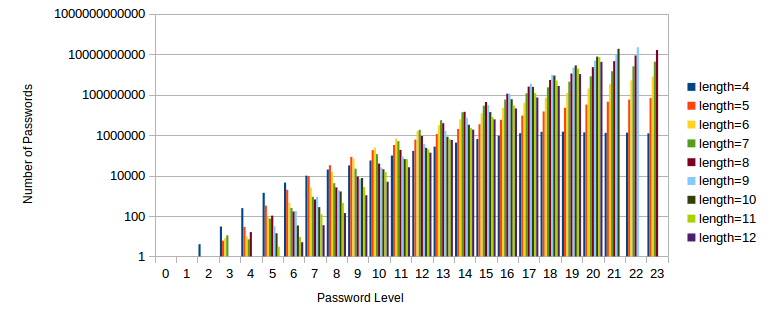
\includegraphics[width=.85\textwidth]{diag/passwd-count.png}
        \end{center}
        \vspace{-15pt}
        \caption{Number of Generated Passwrods for (length,level)-Pairs}
        \label{fig:passnum}
        \end{figure}
    
    \item For a fixed \texttt{length}, the time required to enumerate cases with a certain password level is exponential with respect to \texttt{level}, as shown in Figure \ref{fig:passtime} below. This can be explained by the fact that there are exponentially many of ways to decompose \texttt{level} into a sequence of $(n-k+2)$ numbers, and our algorithm goes through these decompositions regardless if there exists a password  that matches the pattern.

        \begin{figure}[!htbp]
        \begin{center}
            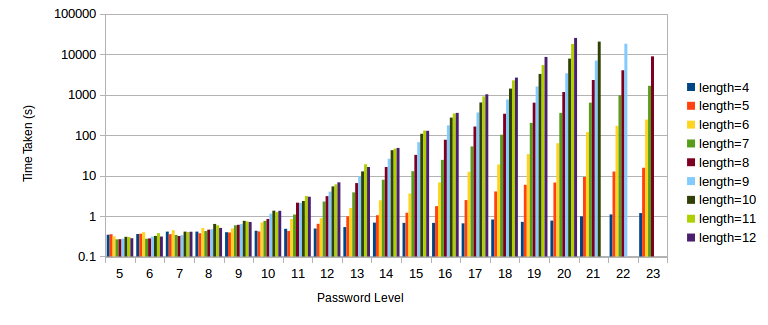
\includegraphics[width=.85\textwidth]{diag/passwd-time.png}
        \end{center}
        \vspace{-15pt}
        \caption{Time Needed to Enumerate (length,level)-Pairs}
        \label{fig:passtime}
        \end{figure}
    
    \item For a fixed \texttt{length}, the \emph{enumeration throughput}, i.e. number of passwords generated per second, rises steadily up to some level, fluctuates around the peak, and then declines, as shown in Figure \ref{fig:passrate}. In general, the trend makes sense because when \texttt{level} is very low or very high, there aren't many passwords but still many potential cases to go over -- and hence the low throughput at the two extremes. Meanwhile, we are not clear about the reason for fluctuations of enumeration throughput around the peak (e.g. for \texttt{length=6}). Our hypothesis is that the ``\texttt{level=20}'' mark allows more wild-card prefix and transition cases in passwords, thereby generating lots of ``cheap'' guesses by simple iteration through $\Sigma^{k-1}$ and $\Sigma$, respectively.
    
        \begin{figure}[!htbp]
        \begin{center}
            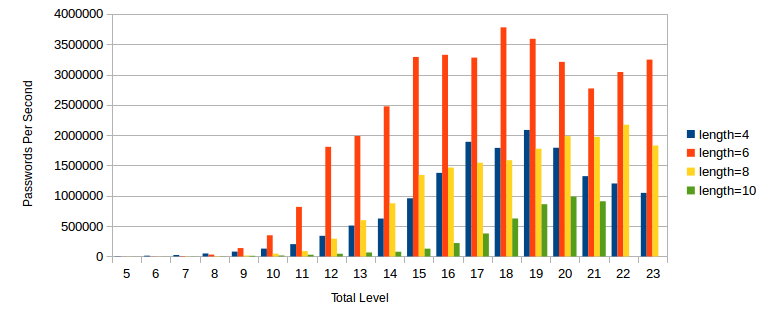
\includegraphics[width=.85\textwidth]{diag/passwd-speed.png}
        \end{center}
        \vspace{-15pt}
        \caption{Enumeration Throughput for (length,level)-Cases}
        \vspace{-15pt}
        \label{fig:passrate}
        \end{figure}
\end{enumerate}

\par\quad Overall, we put lots of analysis on this module since this is the core of our algorithm and is also the performance bottleneck. While running this module on our server, the longest time we tolerated was 426 minutes, i.e. more than seven hours. By projection, all cases we did not cover (shown as ``\texttt{-}'' in Appendix A) would take at least $15$ hours to run, and we decided not to wait for those cases as they do not provide any more insights to the performance of this module.
\par\quad As an ending note, the memory footprint of this module is surprisingly low -- the peak memory for the largest case we covered is capped at 700MB, most of which used to store the actual checkpoints instead of data structures for depth-first search. Thus, the bottleneck for this round is mainly \emph{computational}.


\subsubsection{Calculation Module}
\par\quad Given the result of the previous two modules, this module performs a binary search on the checkpoints, resumes depth-first search from the nearest checkpoint, and returns the guess number very quickly. In our experiments, all queries were fulfilled within one second without causing large memory and computational footprint. Instead of focusing on the benchmark of this module, it is more interesting to examine its results.

\par\quad We built a simple command-line interface for the calculator as in Figure \ref{fig:calculator}, and we are able to feed candidate passwords into the calculator and receive immediate feedback on its guess-number. In Table \ref{table:calcresult1}, and Table \ref{table:calcresult2}, we list some sample results from the calculator. The results are reassuring because they confirm the common wisdom about password security -- for example, adding a digit after ``\texttt{secure}'' caused a 40x in guess number; adding random characters after a very common sequence ``\texttt{123456}'' raised the guess number by six orders of magnitude; mixing upper and lower case letters in ``\texttt{banana}'' caused the guess number to increase by more than 2000x; replacing characters in a common phrase ``\texttt{applepie}'' led to a password outside the range of our 249 billion checkpoints.

\par\quad Hence, we have indirectly shown that our resulting password model is working as intended. 

        \begin{figure}[!htbp]
        \begin{center}
            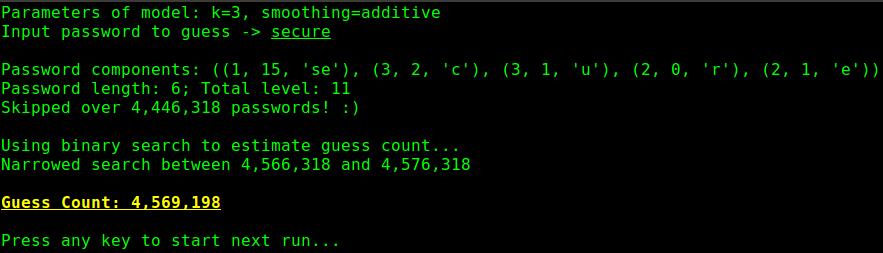
\includegraphics[width=.85\textwidth]{diag/calculator.png}
        \end{center}
        \vspace{-10pt}
        \caption{Command-Line Interface for Guess Number Calculator}
        \label{fig:calculator}
        \end{figure}

    \begin{table}[!htbp]
        \begin{minipage}{.5\linewidth}
            \centering
            \begin{tabular}{|r|r|}
                \hline
                Password:               & Guess Number:                      \\ \hline
                \texttt{secure}         & \texttt{4,569,198}         \\ \hline
                \texttt{123456}         & \texttt{1,693}         \\ \hline
                \texttt{banana}         & \texttt{1,354,764}        \\ \hline
                \texttt{applepie}       & \texttt{715,258,448}         \\ \hline
            \end{tabular}
            
            \caption{Benchmark for \texttt{statgen.py}}
            \label{table:calcresult1}
        \end{minipage}
        %
        \begin{minipage}{.5\linewidth}
            \centering
            \begin{tabular}{|r|r|}
                \hline
                Password:               & Guess Number:                      \\ \hline
                \texttt{secure1}        & \texttt{183,195,279}         \\ \hline
                \texttt{123456yzk}      & \texttt{2,439,725,084}         \\ \hline
                \texttt{baNanA}         & \texttt{3,183,158,806}        \\ \hline
                \texttt{appl3pi3}       & \texttt{> 249,634,722,056}         \\ \hline
            \end{tabular}
            
            \caption{Benchmark for \texttt{statgen.py}}
            \label{table:calcresult2}
        \end{minipage}
    \end{table}
   
\subsection{Computational \& Model Limitations}   \label{sect:limitation}
\par\quad As shown by previous studies, even though the enumeration method based on Markov chain gives a higher rate of success, it is very resource-intensive compared to the other models \cite{guessability}. In our study, we were able to ``checkpoint'' over $3\times 10^{11}$ passwords in around $35$ hours of single-CPU time, and it was infeasible for us to go beyond that since the run-time of checkpoint algorithm rises exponentially against password level (as shown in Table \ref{table:passtime}). Moreover, such computational barrier occurs to our model even for $k=3$. In a more realistic model, a larger value of $k$ is preferred, and thus more computational resources would be necessary.

\par\quad Also, we picked the alphabet for our model to be \emph{alphanumeric characters} in order to reduce the number of parameters. As a result, the password we are able to test are also limited to alphanumeric cases, which is certainly not ideal for real-world usage. Future password security studies should definitely take into account some, if not all, special characters for maximum password coverage. 

\par\quad Eventually, we wish to note that the goal of our implementation is \emph{not} to complete with the performance of professional implementations (like JtR Markov mode), but to gain initial exposure to the field of password security and implement our novel solution based on what we learned from existing literatures and prior algorithm knowledge. Therefore, the guess efficiency of our model might be worse than that of JtR Markov mode, but our design and implementation of the look-up table is completely novel (to the best of our knowledge).
%%%%%%%%%%%%%%%%%%%%%%%%%%%%%%%%%%%%%%%%%%%%%%%%%%%%%%%%%%%%%%%%%%%%
%%%%%%%%%%%%%%%%%%%%%%%%%%%%%%%%%%%%%%%%%%%%%%%%%%%%%%%%%%%%%%%%%%%%
\section{Summary of Findings \& Generalization}
\par\quad In this project, we designed and implemented an efficient Markov-based look-up table that returns the \emph{guess number} of any password very efficiently. Overall, the performance of our model exceeds that of any state-of-the-art Markov enumeration methods, and we validated that the heuristic we chose is reasonable. Meanwhile, there are several key takeaways from our study that we like to mention, as follows:
\begin{itemize}
    \item Time-Space Tradeoff: The key philosophy of our algorithm is based on \emph{time-space tradeoff}, originally proposed in \cite{timespace} in the field of password security. The idea is to reduce the run-time of an algorithm by using more storage space. Our project is the first known effort in applying time-space tradeoff to ordered Markov enumerators in order to support efficient guess number calculation.
    \vskip 2pt
    \par While designing our algorithm, we noticed that probabilistic models for passwords tend to have a huge number of states and parameters in general, and it would almost always help if some \emph{pre-processing work} (e.g. \emph{Checkpointing module} in our case) is done to reduce \emph{repeated work}. For example, in our checkpointing algorithm, we traverse the password search tree (Figure \ref{fig:checkpoint}) \emph{only once} and save checkpoints on the hard drive for later use. Similar approach can be used for PCFG and even word-mangling rule for efficient guess-number calculation.
    
    \item Discretization: Another efficient measure that reduces the complexity of our algorithm is \emph{discretization}, by which we approximate continuous variables with discrete states in order to allow easier optimization, traversal, and calculation. We discovered that discretization is key to the viablity of our algorithm, as it is practically impossible to keep track of trillions of accurate password probabilities. For future research on probabilistic password models, discretization can be an invaluable asset in reducing the problem state by sacrificing some accuracy.
    
    \item Bottleneck Analysis \& Parallelism: Since we already predicted that Markov enumeration algorithms use significant resources, we studied which types of resources are the bottlenecks at each step. We concluded that in the training phase, the bottleneck was memory, which needs to store the $k$-gram statistics and probability values; in the checkpointing phase, the bottleneck was CPU time since performing depth-first search on the huge password tree involves a huge amount of work. And, the latter observation prompted us to look into parallelization techniques available for our algorithm, and we achieved 10x speedup by using parallelism.

\end{itemize}

%%%%%%%%%%%%%%%%%%%%%%%%%%%%%%%%%%%%%%%%%%%%%%%%%%%%%%%%%%%%%%%%%%%%
%%%%%%%%%%%%%%%%%%%%%%%%%%%%%%%%%%%%%%%%%%%%%%%%%%%%%%%%%%%%%%%%%%%%
\section{Further Work \& Enhancements}

\par\quad Considering that we were newly introduced to the field of password security three months ago and that this is only a semester-long project, the amount of work we could have done is limited. Although our password guess count calculator gives great results, it does have many areas for improvement. In this section, we discuss the top items in our wishlist, and hope that they can provide directions for future research in the same area.

\subsection{Improvements on Markov Model}
\par\quad The Markov model used in our project is the classic model as shown in Figure \ref{fig:markov}. Meanwhile, alternatives including \emph{layered Markov model} can be used for our purpose, as shown in Figure \ref{fig:layered} below. The main caveat with the layered model is that there are more parameters to learn, so special attention is needed to address sparseness and prevent overfitting.

    \begin{figure}[!htbp]
        \vspace{-15pt}
        \begin{center}
            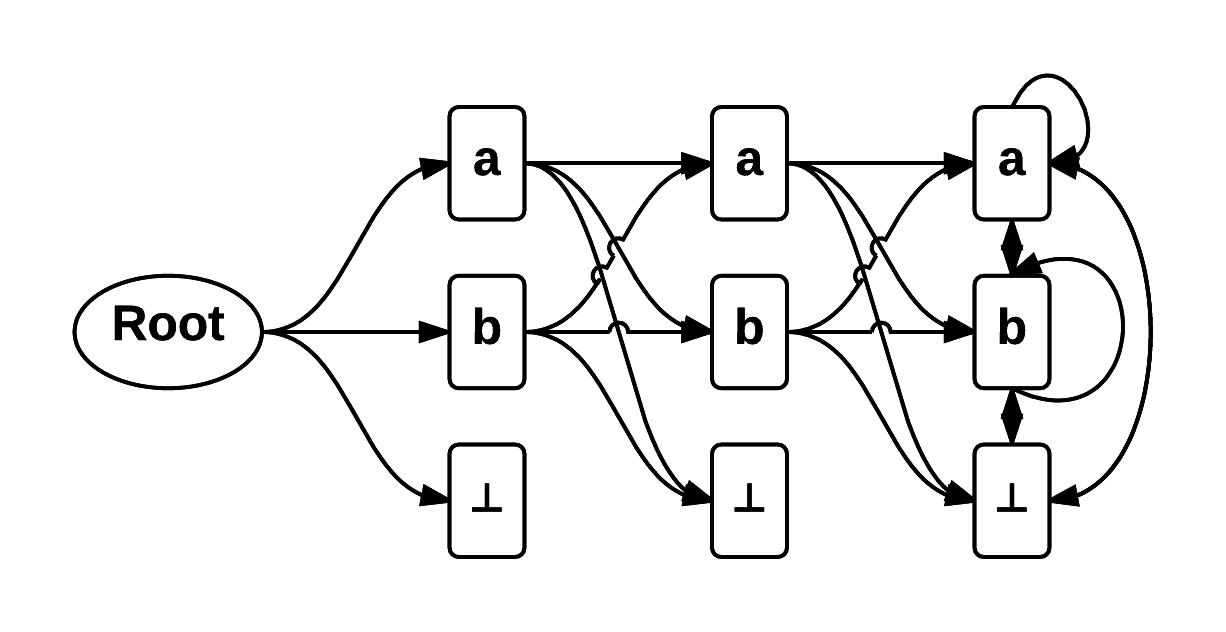
\includegraphics[width=.6\textwidth]{diag/layered-markov.png}
        \end{center}
        \vspace{-15pt}
        \caption{Sample of Layered Markov Model}
         \vspace{-5pt}
        \label{fig:layered}
    \end{figure}

\par\quad As for the \emph{smoothing technique} for our model, we applied \emph{additive smoothing} to $k$-gram counts in Algorithm \ref{algo:probgen}. Meanwhile, other more complicated techniques can be used -- an example is \emph{Good-Turing smoothing}. Instead of adjusting the $k$-gram counts, this technique \emph{pre-processes the dataset} $\mathcal{D}$ even before we feed it to the statistics generation routine (\texttt{statgen}) -- the smoothing routine adjusts the \emph{count} of each entry, i.e. $c(s)$ for $s\in\Sigma^L$ as follows:
\vspace{-5pt}
$$\hat{c}(s) = \begin{cases}
             0.22       & \text{for } c(s) = 1  \\
             0.88       & \text{for } c(s) = 2  \\
             c(x) - 1   & \text{for } c(s) > 2  \\
             \dfrac{\sum_{s\in\Sigma^L}{(c(s) - \hat{c}(s))}}{|\{s\in\Sigma^L \mid {c(s)=0}\}}  & \text{otherwise}
         \end{cases},\vspace{-1pt}
$$
where the last case above simply means to uniformly distribute the deducted count values to unobserved passwords in the universe $\Sigma^L$. After adjusting the counts, the \emph{(password, count)} pairs are then passed to \texttt{statgen} (Algorithm \ref{algo:statgen}) and then to \texttt{probgen} (Algorithm \ref{algo:probgen}) with $\delta = 0$ (i.e. no additive smoothing applied).

\par\quad As an ending note on the \emph{training dataset} for our model, we only included RockYou database and Unix English dictionary as noted in \ref{sect:data-analysis}. While they constitute a satisfactory training set, more weighted training sets can be used to improve the accuracy of our model. Also, a larger value of $k$ ($4$ or $5$) will likely result in a more efficient guessing model according to \cite{probabilistic}.

\subsection{Password Strength Meter / Guessability-as-a-Service}
\par\quad Given our efficient algorithm for calculating guess numbers, we believe it can be an useful addition to existing password meters (e.g. Google checker). After enforcing the character composition rules for screening purposes, the password checker may feed the password to our algorithm and estimate its strength based on its guess number. With proper tuning of the underlying Markov model (as in previous section) and our efficient algorithm, Markov-based password checkers have the potential to become the new mainstream methodology. Similarly, our algorithm may also be used to complement existing Markov enumeration methods in password guessability services (such as \cite{cmu-guessability}) to speed up the calculation.

\vskip .3in
\section*{Acknowledgements}
\par\quad The authors thank our advisors Lujo Bauer and Blase Ur for proposing the research topic and holding regular meetings to track our progress and review our report. We also thank Blase Ur for pointing us to many of the references, which introduced us to the area of password security.

%%%%%%%%%%%%%%%%%%%%%%%%%%%%%%%%%%%%%%%%%%%
%%% References
%%%%%%%%%%%%%%%%%%%%%%%%%%%%%%%%%%%%%%%%%%%
\urlstyle{rm}
\vskip .2in
\begin{thebibliography}{9}

\bibitem{adaptive markov}
C. Castelluccia, M. D\"{u}umuth,  and D. Perito. Adaptive password-strength meters from Markov models. In \textit{Proc. NDSS}, 2012.

\bibitem{cmu-guessability}
Carnegie Mellon University. Password guessability service. \url{https://pgs.ece.cmu.edu}, 2015.

\bibitem{entropy}
D. Davis, F. Monrose, M. K. Reiter. On user choice in graphical password schemes. \emph{Proceedings of the 13th conference on USENIX Security Symposium}, 2004.

\bibitem{empirical}
M. Dell’Amico, P. Michiardi, and Y. Roudier. Password strength: an empirical analysis. In \textit{INFOCOM}, pp. 1-9, 2010.

\bibitem{omen}
M. D\"{u}rmuth, F. Angelstorf, C. Castelluccia, D. Perito, and A. Chaabane. OMEN: faster password guessing using an ordered markov enumerator. In \textit{Proc. ESSoS}, 2015.

\bibitem{money}
D. Flor\^{e}ncio and C. Herley. Is everything we know about password-stealing wrong? \textit{IEEE Security \& Privacy Magazine}, DOI 10.1109/MSP.2012.57, 2012.

\bibitem{mangled2}
A. Forget, S. Chiasson, P. Van Oorschot, and R. Biddle. Improving text passwords through persuasion. In \emph{Proc. SOUPS (2008)}.

\bibitem{probframework}
J. Galbally, I. Coisel, and I. Sanchez. A probabilistic framework for improved password strength metrics. In \textit{Proc. International Carnahan Conference on Security Technology (ICCST)},  pp. 1-6, 2014.

\bibitem{good-turing}
W. A. Gale and G. Sampson. Good-turing frequency estimation without tears. \emph{Journal of Quantitative Linguistics}, 2(1);217-237, 1995.

\bibitem{google-ngram}
Google. Google ngram viewer. \url{https://books.google.com/ngrams/info}, 2010-.

\bibitem{SQL injection}
W. G. Halfond, J. Viegas, and A. Orso. A classification of SQL-injection attacks and countermeasures. In \textit{Proc. of the Intl. Symposium on Secure Software Engineering}, Mar. 2006.

\bibitem{persistence}
C. Herley and P.C. van Oorschot. A research agenda acknowledging the persistence of passwords. \textit{IEEE Security \& Privacy}, 10(1):28-36, 2012.

\bibitem{PKCS}
B. Kaliski. PKCS \#5: Password-based cryptography specification, RFC 2898. The Internet Society, 2000.

\bibitem{againagain}
P. G. Kelley, S. Komanduri, M. L. Mazurek, R. Shay, T. Vidas, L. Bauer, N. Christin, L. F. Cranor, and J. Lopez. Guess again (and again and again): Measuring password strength by simulating password-cracking algorithms. In \textit{Proc. IEEE Symposium on Security and Privacy}, 2012.

\bibitem{pcfg}
D. Klein and C. D. Manning. Accurate Unlexicalized Parsing. \emph{Proceedings of the 41st Meeting of the Association for Computational Linguistics}, pp. 423-430. 2003.

\bibitem{probabilistic}
J. Ma, W. Yang, M. Luo, and N. Li. A study of probabilistic password models. In \textit{Proc. IEEE Symp. on Security and Privacy}, 2014.

\bibitem{moore}
G. E. Moore. No exponential is forever: but ``forever'' can be delayed! \emph{International Solid State Circuits Conference}, 2003. 

\bibitem{history}
R. Morris and K. Thompson. Password security: a case history. \emph{Commun. ACM}, 22(11):594-597, 1979.

\bibitem{timespace}
A. Narayanan and V. Shmatikov. Fast dictionary attacks on passwords using time-space tradeoff. In \textit{Proc. 12th ACM conference on Computer and Communications Security (CCS)}, pp. 364 - 372, 2005.

\bibitem{bcrypt}
P. Niels and D. Mazi\`{e}res. A future-adaptable password scheme. In \emph{Proc. USENIX}, 1999.

\bibitem{john}
OpenWall. John the Ripper, 2012. \url{http://www.openwall.com/john}.

\bibitem{john-benchmark}
Openwall. John the Ripper benchmarks. Internet: \url{http://openwall.info/wiki/john/benchmarks}, Aug. 1, 2015 [Nov. 27, 2015].

\bibitem{john-markov}
OpenWall. Markov Generator. Internet: \url{http://openwall.info/wiki/john/markov}, Mar. 29, 2010 [Nov. 28, 2015].

\bibitem{scrypt}
C. Percival. Stronger key derivation via sequential memory-hard functions. \textit{BSDCan}, 2009

\bibitem{easypass}
E. H. Spafford. OPUS: Preventing weak password choices. \textit{Computers and Security}, 11(3) pp.273-278, 1992.

\bibitem{hashcat-mask}
J. Steube. Mask attack. Internet: \url{https://hashcat.net/wiki/doku.php?id=mask_attack}, 2009-.

\bibitem{hashcat-markov}
J. Steube. statsprocessor. Internet: \url{https://hashcat.net/wiki/doku.php?id=statsprocessor}, 2009-.

\bibitem{passmodel}
W. Tansey. Improved Models for Password Guessing. University of Texas, \textit{Tech. Rep.}, 2011.

\bibitem{measureup}
B. Ur, P. G. Kelley, S. Komanduri, J. Lee, M. Maass, M. Mazurek, T. Passaro, R. Shay, T. Vidas, L. Bauer, N. Christin, and L. F. Cranor. How does your password measure up? The effect of strength meters on password creation. In \emph{Proc. USENIX Security}, 2012

\bibitem{addbang}
B. Ur, F. Noma, J. Bees, S. Segreti, R. Shay, L. Bauer, N. Christin, and L.F. Cranor. ``I added ’!’ at the end to make it secure'': Observing password creation in the lab. In \textit{Symposium on Usable Privacy and Security (SOUPS)}. USENIX, 2015.

\bibitem{guessability}
B. Ur, S. M. Segreti, L. Bauer, N. Christin, L. F. Cranor, S. Komanduri, D. Kurilova, M. L. Mazurek, W. Melicher, and R. Shay. Measuring real-world accuracies and biases in modeling password guessability. In \textit{Proc. USENIX Security}, 2015.

\bibitem{PCFG}
M. Weir, S. Aggarwal, B. de Medeiros, and B. Glodek. Password cracking using probabilistic context-free grammars. In \emph{IEEE Symposium on Security and Privacy}, pp. 391-405, 2009.

\bibitem{pcfg-smoothing}
S. H. Yazdi. \emph{Probabilistic Context-Free Grammar Based Password Cracking: Attack, Defense and Applications}. PhD thesis, Florida State University, 2015.
\end{thebibliography}

%%%%%%%%%%%%%%%%%%%%%%%%%%%%%%%%%%%%%%%%%%%
%%% Appendices
%%%%%%%%%%%%%%%%%%%%%%%%%%%%%%%%%%%%%%%%%%%
\vspace{\fill}
\pagebreak


\newgeometry{top=.65in,bottom=.65in, left=.8in, right=.8in}
\section*{Appendices}
\subsection*{Appendix A: Benchmark for Checkpoint Generation (Section \ref{sect:lookup})}
\par\quad In this appendix, we show the total password count for different length and password levels, and also the time taken to generate each password checkpoint file. As in the report, our input data file is processed with with $k=3$ and \emph{additive smoothing}. And, the \texttt{checkpoint\_interval} for our runs is 10,000. Overall, over $3\times 10^{11}$ passwords are generated in over 35 hours, and the maximal RAM usage for each routine ranges between 100 MB - 700 MB depending on its size.
    \begin{table}[!htbp]
        \vspace{-5pt}
        \footnotesize
        \begin{center}
        \setlength{\tabcolsep}{3.5pt}
            \begin{tabular}{|c||r|r|r|r|r|r|r|r|r|}
                \hline
                lvl{\bf\textbackslash}len: & 4 & 5 & 6 & 7 & 8 & 9 & 10 & 11 & 12 \\ \hline \hline

                0 & 1 & 1 & 1 & 0 & 0 & 0 & 0 & 0 & 0  \\\hline
                1 & 0 & 0 & 0 & 1 & 0 & 0 & 0 & 0 & 0  \\\hline
                2 & 4 & 1 & 0 & 0 & 1 & 0 & 0 & 0 & 0  \\\hline
                3 & 30 & 6 & 8 & 11 & 0 & 1 & 0 & 0 & 0 \\\hline
                4 & 244 & 29 & 10 & 7 & 16 & 0 & 0 & 0 & 0 \\\hline
                5 & 1405 & 325 & 85 & 74 & 104 & 31 & 14 & 3 & 1 \\\hline
                6 & 4472 & 1973 & 445 & 250 & 166 & 174 & 34 & 9 & 5 \\\hline
                7 & 9887 & 9441 & 2599 & 896 & 654 & 879 & 274 & 121 & 35 \\\hline
                8 & 19856 & 32588 & 14905 & 4171& 2593 & 1894 & 1630 & 442 & 139 \\\hline
                9 & 31765 & 84334 & 68047 & 21901 & 8978 & 6777 & 7597 & 2667 & 1062 \\\hline
                10 & 56258 & 181813 & 243625 & 115153 & 39027 & 24952 & 20531 & 15073 & 4921 \\\hline
                11 & 98139 & 327151 & 688308 & 507085 & 187860 & 87282 & 65175 & 65811 & 25623\\\hline
                12 & 166549 & 603670 & 1596876 & 1856345 & 908434 & 359444 & 236917 & 199618 & 135660\\\hline
                13 & 272504 & 1133645 & 3134553 & 5501241 & 3899639 & 1608764 & 837871 &  635539& 583632\\\hline
                14 & 429877 & 2033392 & 6071992 & 13560299 & 14320603 & 7328242 & 3280402 & 2232286& 1886267 \\\hline
                15 & 649264 & 3477273 & 11917118 & 28687867 & 43887833 & 30631783 & 13914607 & 7903573 & 6085586 \\\hline
                16 & 936124 & 5788039 & 22510339 & 58265504 & 113343934 & 112288927 & 60248304 & 29819178 & 20920106 \\\hline
                17 & 1248219 & 9421256 & 40687870 & 118476973 & 253921885 & 351289423 &  245096824 & 121062142 & 73395729 \\\hline
                18 & 1471896 & 14838699 & 71423060 & 233963339 & 538919236 & 939203528 & 892537472 & 502365205 & 270423230 \\\hline
                19 & 1498136 & 22517047 & 122446171 & 443550818 & 1133062727 & 2201509486 & 2826265452 & 1991368176 & 1058337629 \\\hline
                20 & 1380619 & 32781103 & 204019986 & 815544166 & 2324086410 & 4854945013 & 7754190749 & 7183645342 & 4236844144 \\\hline
                21 & 1300991 & 45127607 & 330517903 & 1462702804 & 4593181179 & 10525767778 & 18838039024 & \texttt{-} & \texttt{-} \\\hline
                22 & 1323190 & 58001173 & 521059245 & 2555448779 & 8794461087 & 22310905515 & \texttt{-} & \texttt{-} & \texttt{-} \\\hline
                23 & 1239847 & 68874676 & 793986509 & 4353125874 & 16406818888 & \texttt{-} & \texttt{-} & \texttt{-} & \texttt{-} \\\hline
            \end{tabular}
        \end{center}
        \vspace{-5pt}
        \caption{Password Count for (length,level)-Pairs}
        \label{table:passcount}
    \end{table}

    \begin{table}[!htbp]
        \vspace{-5pt}
        \footnotesize
        \begin{center}
        \setlength{\tabcolsep}{3.5pt}
            \begin{tabular}{|c||r|r|r|r|r|r|r|r|r|}
                \hline
                lvl{\bf\textbackslash}len: & 4 & 5 & 6 & 7 & 8 & 9 & 10 & 11 & 12 \\ \hline \hline
                5 &0.345s &0.355s &0.315s &0.265s &0.267s &0.276s &0.307s &0.302s &0.283s \\\hline
                6 &0.359s &0.365s &0.400s &0.275s &0.280s &0.310s &0.322s &0.378s &0.311s \\\hline
                7 &0.413s &0.355s &0.447s &0.339s &0.320s &0.337s &0.413s &0.403s &0.409s \\\hline
                8 &0.412s &0.376s &0.503s &0.425s &0.461s &0.472s &0.638s &0.590s &0.507s \\\hline
                9 &0.399s &0.393s &0.492s &0.590s &0.608s &0.634s &0.759s &0.733s &0.713s \\\hline
                10 &0.434s &0.416s &0.697s &0.759s &0.848s &1.143s &1.357s &1.251s &1.350s \\\hline
                11 &0.483s &0.426s &0.842s &1.088s &2.136s &2.107s &2.353s &3.118s &3.000s \\\hline
                12 &0.490s &0.643s &0.883s &2.286s &3.103s &4.013s &5.416s &6.057s &6.824s \\\hline
                13 &0.535s &0.982s &1.577s &3.859s &6.533s &9.677s &12.705s & 19.065s &16.367s \\\hline
                14 &0.688s &1.049s &2.453s &7.896s &16.335s &26.163s &42.602s &46.728s &48.509s \\\hline
                15 &0.677s &1.208s &3.621s &12.880s &32.660s &1m7.558s &1m48.478s &2m10.373s &2m8.807s \\\hline
                16 &0.679s &1.758s &6.768s &24.603s &1m17.340s & 2m55.354s & 4m33.393s & 5m44.745s & 5m57.467s \\\hline
                17 &0.660s &2.480s &12.406s &52.846s & 2m44.362s & 6m6.055s &  10m46.765s & 15m12.206s & 17m9.454s \\\hline
                18 &0.822s &4.056s &18.900s &1m43.318s & 5m39.574s & 12m46.142s & 23m46.444s & 37m59.829s & 44m24.053s \\\hline
                19 &0.718s &5.923s &34.115s & 3m22.496s & 10m37.857s & 26m51.188s & 54m40.751s & 90m37.299s & 144m13.870s \\\hline
                20 &0.770s &6.755s &1m3.572s & 5m56.899s & 19m31.302s & 56m55.179s & 130m59.616s & 304m2.714s & 426m4.180s \\\hline
                21 &0.983s &9.266s &1m59.264s & 10m39.659s & 38m48.328s & 117m14.942s & 345m13.088s & \texttt{-} & \texttt{-} \\\hline
                22 &1.100s &12.592s & 2m51.269s & 16m16.114s & 67m27.478s & 305m52.786s & \texttt{-} & \texttt{-} & \texttt{-} \\\hline
                23 &\;\; 1.183s & \;\; 15.659s & 4m4.550s & 27m49.799s & 149m19.359s & \texttt{-} & \texttt{-} & \texttt{-} & \texttt{-} \\\hline
            \end{tabular}
        \end{center}
        \vspace{-5pt}
        \caption{Run-Time for Checkpointing (length,level)-Cases}
        \label{table:passtime}
    \end{table}

\vspace{\fill}
\pagebreak
\subsection*{Appendix B: Selected Source Code for Algorithm \ref{algo:probgen} (\texttt{probgen}) \protect\footnote{This and all following source code is available on our project Github page: \url{https://github.com/ymzong/password-guessability}.}}

\begin{python}
def report_probability(StartCount, MidCount, EndCount, is_smoothed, delta):
    smooth_str = "additive" if is_smoothed else "none"

    # For starting probability
    tmp_dict = defaultdict(lambda: 0)
    dict_sum = sum(StartCount.values())
    new_sum = dict_sum + delta * ALPHABET_SIZE ** (k - 1)
    for pref in StartCount:
        tmp_dict[pref] = (StartCount[pref] + delta) * 1.0 / new_sum
    if is_smoothed:
        tmp_dict[""] = delta * 1.0 / new_sum # Pseudo-count for non-existent prefix

    outfile = os.path.join(
        CURRENT_DIR, "../data/probs/{}_{}_start.json".format(k, smooth_str))
    print("Writing output to {}...".format(outfile)),
    with open(outfile, 'w') as f:
        json.dump(tmp_dict, f, sort_keys=True, indent=4)
    print("Done!")
    del(tmp_dict)

    # For ending probability
    tmp_dict = defaultdict(lambda: 0)
    dict_sum = sum(EndCount.values())
    new_sum = dict_sum + delta * ALPHABET_SIZE ** (k - 1)
    for suff in EndCount:
        tmp_dict[suff] = (EndCount[suff] + delta) * 1.0 / new_sum
    if is_smoothed:
        tmp_dict[""] = delta * 1.0 / new_sum # Pseudo-count for non-existent suffix

    outfile = os.path.join(
        CURRENT_DIR, "../data/probs/{}_{}_end.json".format(k, smooth_str))
    print("Writing output to {}...".format(outfile)),
    with open(outfile, 'w') as f:
        json.dump(tmp_dict, f, sort_keys=True, indent=4)
    print("Done!")
    del(tmp_dict)

    # For transition probability
    tmp_dict = defaultdict(lambda: defaultdict(lambda: 0))
    for pref in MidCount:
        dict_sum = sum(MidCount[pref].values())
        new_sum = dict_sum + delta * ALPHABET_SIZE
        for next_chr in MidCount[pref]:
            tmp_dict[pref][next_chr] = MidCount[pref][next_chr] * 1.0 / new_sum

        if is_smoothed:
            tmp_dict[pref][""] = delta * 1.0 / new_sum  # Ditto

    # Write to output file
    outfile = os.path.join(
        CURRENT_DIR, "../data/probs/{}_{}_mid.json".format(k, smooth_str))
    print("Writing output to {}...".format(outfile)),
    with open(outfile, 'w') as f:
        json.dump(tmp_dict, f, sort_keys=True, indent=4)
    print("Done!")
\end{python}

\vspace{\fill}
\pagebreak
\subsection*{Appendix C: Selected Source Code for Checkpoint Generation (Section \ref{sect:lookup})}

\begin{python}
def dfs_passwords(l, k, next_idx, passwd, remaining_lvl):
    global GUESS_COUNT
    global CHECKPOINT

    # Finishing case
    if next_idx == l:   # End of password
        # Verify ending level matches
        # if passwd[-(k-1):] in end_lvl[remaining_lvl]:
        if remaining_lvl == 0:
            GUESS_COUNT += 1
            if GUESS_COUNT % UPDATE_FREQUENCY == 0:
                CHECKPOINT.append(passwd)
        return
    # Trim impossible cases
    elif MAX_LEVEL * (l - next_idx) < remaining_lvl:
        return
    # Last character
    elif next_idx == l - 1:
        suffix = passwd[-(k - 1):]
        if suffix not in mid_lvl:
            if remaining_lvl != NEXT_CHR_LVL:
                return
            for c in ALPHABET:
                GUESS_COUNT += 1
                if GUESS_COUNT % UPDATE_FREQUENCY == 0:
                    CHECKPOINT.append(passwd + c)
        elif remaining_lvl not in mid_lvl[suffix]:
            return  # Ehh, bad case
        for next_chr in mid_lvl[suffix][remaining_lvl]:
            if next_chr != "":
                GUESS_COUNT += 1
                if GUESS_COUNT % UPDATE_FREQUENCY == 0:
                    CHECKPOINT.append(passwd + next_chr)
            else:
                for c in ALPHABET:
                    if c in mid_tokens[suffix]:
                        continue
                    GUESS_COUNT += 1
                    if GUESS_COUNT % UPDATE_FREQUENCY == 0:
                        CHECKPOINT.append(passwd + c)
    # Initial case
    elif next_idx == 0:
        for init_level in xrange(0, min(remaining_lvl, MAX_LEVEL)):
            if init_level not in start_lvl:
                continue
            for init_sequence in start_lvl[init_level]:
                if init_sequence != "":
                    # Normal case
                    dfs_passwords(l, k, k - 1, init_sequence, remaining_lvl - init_level)
                else:
                    # Wildcard case...
                    for init_seq in ("".join(k) for k in itertools.product(ALPHABET, repeat=k-1)):
                        if init_seq in start_tokens:
                            continue
                        dfs_passwords(l, k, k - 1, init_seq, remaining_lvl - init_level)
    # Intermediate case
    else:
        prefix = passwd[-(k - 1):]
        if prefix not in mid_lvl:
            # Special case when we apply uniform probability to everything
            for c in ALPHABET:
                dfs_passwords(l, k, next_idx + 1, passwd + c, remaining_lvl - NEXT_CHR_LVL)
            return
        # Regular case
        for next_level in xrange(0, min(remaining_lvl, MAX_LEVEL)):
            if next_level not in mid_lvl[prefix]:
                continue
            for next_chr in mid_lvl[prefix][next_level]:
                # Wildcard case...
                if next_chr == "":
                    for c in ALPHABET:
                        if c in mid_tokens[prefix]:
                            continue
                        dfs_passwords(l, k, next_idx + 1, passwd + c, remaining_lvl - next_level)
                # Normal case
                else:
                    dfs_passwords(l, k, next_idx + 1, passwd + next_chr, remaining_lvl - next_level)
\end{python}

\vspace{\fill}
\pagebreak
\subsection*{Appendix D: Selected Source Code for Algorithm \ref{algo:newpassenum} (\texttt{new-passenum})}

\begin{python}
def decompose_password(pw, k):
    result = ()

    # Level for prefix
    prefix = pw[:(k - 1)]
    found = False
    index = -1
    for l in start_lvl:
        if prefix in start_lvl[l]:
            found = True
            index = start_lvl[l].index(prefix)
            break
    # Does not appear in index, must be wildcard
    if not found:
        for l in start_lvl:
            if "" in start_lvl[l]:
                index = start_lvl[l].index("")
                break
    assert(index >= 0)
    result += ((l, index, prefix),)

    # Level for intermediate characters
    for i in xrange(0, len(pw) - k + 1):
        prefix = pw[i: i + k - 1]
        # Prefix not in index -- all is wildcard case
        if prefix not in mid_lvl:
            result += ((NEXT_CHR_LVL, ALPHABET.index(pw[i + k - 1]), pw[i + k - 1]), )
            continue
        # Prefix in index -- find corresponding level
        found = False
        index = -1
        for l in mid_lvl[prefix]:
            if pw[i + k - 1] in mid_lvl[prefix][l]:
                found = True
                index = mid_lvl[prefix][l].index(pw[i + k - 1])
                break
        if not found:
            for l in mid_lvl[prefix]:
                if "" in mid_lvl[prefix][l]:
                    index = mid_lvl[prefix][l].index("")
                    break
        assert(index >= 0)
        result += ((l, index, pw[i + k - 1]), )
    return result
\end{python}

\vspace{\fill}
\pagebreak
\subsection*{Appendix E: Handout about Guess Number \& Cracking Time}
    \par\quad We prepared the following handout for the project fair on Dec 10, 2015 in order to demonstrate the correlation between guess number and cracking time.
    \begin{figure}[!htbp]
        \vspace{-60pt}
        \begin{center}
            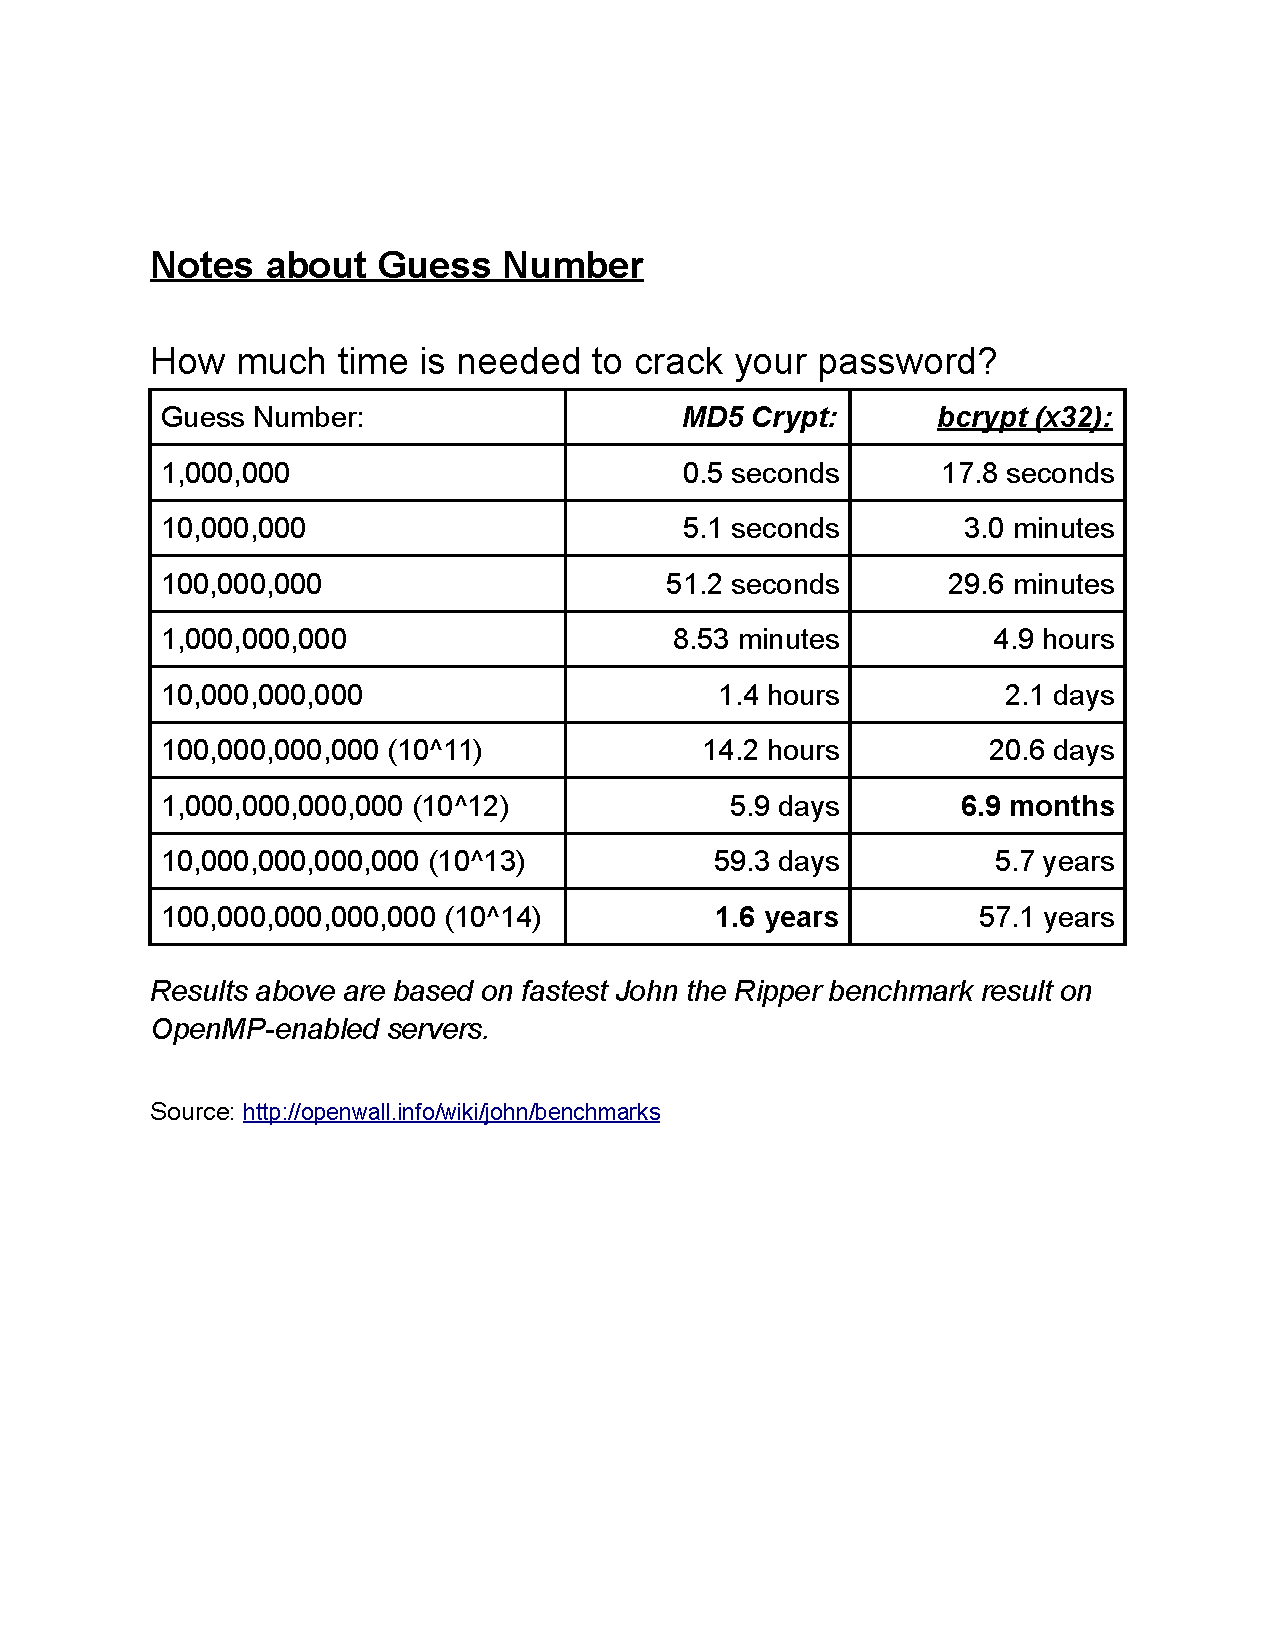
\includegraphics[width=.95\textwidth]{diag/guess-number-handout.pdf}
        \end{center}
        \vspace{-20pt}
        \label{fig:handout}
    \end{figure}

\end{document}
